% =====================================================================
%  Shared sections (model, stability, control, swing-up) used by build_full_report.py and build_phase_reports.py
%  (layout follows the senior reference report: title page, contents,
%   numbered sections, code listings, tabulation, conclusion, contributions)
% =====================================================================
\documentclass[12pt,a4paper]{article}
\usepackage[a4paper,margin=1in]{geometry}
\usepackage[T1]{fontenc}
\usepackage{lmodern}
\usepackage{amsmath,amssymb,bm}
\usepackage{graphicx,float,booktabs,array,multirow}
\usepackage{xcolor}
\usepackage{algorithm}
\usepackage{algpseudocode}
\usepackage{fancyhdr}
\usepackage{enumitem}
\usepackage{caption}
\usepackage[hidelinks]{hyperref}

\pagestyle{fancy}
\fancyhf{}
\renewcommand{\headrulewidth}{0.6pt}
\fancyfoot[C]{\thepage}
\setlength{\headheight}{14.5pt}
\setlength{\parskip}{4pt}
\setlength{\parindent}{0pt}
\newcommand{\Nm}{\,\mathrm{N\,m}}
\captionsetup{font=small}

\begin{document}

\begin{titlepage}
\centering
\vspace*{2cm}

\includegraphics[width=4.2cm]{figures/logo-000.jpg}\\[3cm]
{\Huge Systems Thinking Project}\\[0.5cm]
{\Large Acrobot: Modelling, Stability, Control and Swing-Up}\\[0.25cm]
{\large Full Project Report}\\[2.2cm]
\begin{tabular}{cc}
\textbf{Author:} Bhargav & \textbf{Author:} Sreekar\\
ID: 2025102061 & ID: 2025102074\\[0.8cm]
\textbf{Author:} Kaushik & \textbf{Author:} Divijat\\
ID: 2025102071 & ID: 2025102040
\end{tabular}
\vfill
{\large November 11, 2026}
\end{titlepage}

\tableofcontents
\newpage
% =====================================================================
\section{Introduction}\label{sec:intro}
% =====================================================================
\subsection{What is an Acrobot?}
An acrobot is a two-link pendulum that hangs from a fixed pivot. The first link (the ``shoulder'' link) is free to rotate about the pivot; the second link is joined to the end of the first at the ``elbow''. The only motor sits at the elbow, so the shoulder is \emph{passive}. It is the robot version of a gymnast on a high bar who can only swing the legs at the hips. Because there are two degrees of freedom but only one actuator, the acrobot is a standard example of an \emph{underactuated} system [1], [2].

\subsection{Objective}
The project builds up, step by step, from a model to a robot that swings itself up and balances:
\begin{enumerate}
\item derive and verify the nonlinear model, find every equilibrium, and linearize about each one (Sections~\ref{sec:model}--\ref{sec:lin});
\item determine the stability of every equilibrium from the transfer functions and the state-space model, supported by simulation (Section~\ref{sec:stab});
\item decide whether feedback from a single measured joint angle can stabilize the upright, and explain why (Section~\ref{sec:single});
\item design controllers for the upright and the other equilibria, and characterize how far from each equilibrium they still work with $\tau_{\max}=20\Nm$ (Sections~\ref{sec:ctrl}--\ref{sec:limits});
\item starting from hanging, swing the acrobot up to the upright and hold it, and explain why the controller behaves as it does (Section~\ref{sec:swing});
\item compare the hand-designed swing-up with one learned by reinforcement learning (Section~\ref{sec:rl});
\item rebuild every model and controller (except the learned one) in Simulink and cross-check it against the Python results (Section~\ref{sec:simulink}).
\end{enumerate}

% =====================================================================
\section{System Modelling}\label{sec:model}
% =====================================================================
\subsection{Model}
The configuration is described by two generalised coordinates: $q_1$, the angle of link~1 from the downward vertical, and $q_2$, the angle of link~2 relative to link~1. The full state contains the angles and their rates:
\[
\mathbf q=\begin{bmatrix}q_1\\q_2\end{bmatrix},\qquad
\mathbf x=\begin{bmatrix}q_1\\q_2\\\dot q_1\\\dot q_2\end{bmatrix}.
\]
\begin{figure}[H]
\centering
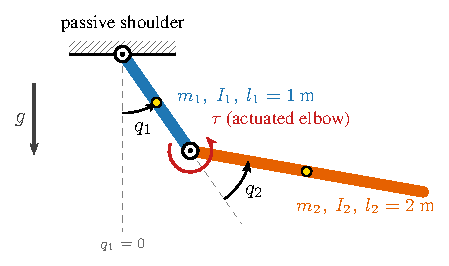
\includegraphics[width=0.42\textwidth]{figures/acrobot_diagram.pdf}
\caption{The acrobot: passive shoulder at the pivot, motor torque $\tau$ at the elbow; dots mark the centres of mass.}
\label{fig:acrobot}
\end{figure}

\subsection{Equations of Motion}
The dynamics (given in the course helper document and verified in Section~\ref{sec:sim}) are
\begin{equation}
M(q)\,\ddot q+C(q,\dot q)\,\dot q=\tau_g(q)+B\,\tau,\qquad B=\begin{bmatrix}0\\1\end{bmatrix},\qquad |\tau|\le 20\Nm .\label{eq:eom}
\end{equation}

\textbf{$\tau$ (Input Torque):} the torque of the elbow motor, the only quantity we command. $B=[0,\,1]^T$ says it acts on the elbow equation only.

\textbf{$M(q)$ (Inertia Matrix):} the resistance to angular acceleration. It depends on the elbow angle because the mass distribution changes as the arm folds:
\begin{equation}
M(q)=\begin{bmatrix}2.663+2\cos q_2 & 1.33+\cos q_2\\ 1.33+\cos q_2 & 1.33\end{bmatrix},\qquad \det M=1.7729-\cos^2q_2\ge0.7729>0 .
\end{equation}

\textbf{$C(q,\dot q)$ (Coriolis Matrix):} the coupling forces between the links (centrifugal and Coriolis effects):
\begin{equation}
C(q,\dot q)=\sin q_2\begin{bmatrix}-2\dot q_2 & -\dot q_2\\ \dot q_1 & 0\end{bmatrix}.
\end{equation}

\textbf{$\tau_g(q)$ (Gravity Torque):} the torque that gravity exerts on each joint, $\tau_g=-\partial U/\partial q$, with potential energy $U$:
\begin{equation}
U=-14.715\cos q_1-9.81\cos(q_1+q_2),\qquad
\tau_g(q)=-9.81\begin{bmatrix}1.5\sin q_1+\sin(q_1+q_2)\\ \sin(q_1+q_2)\end{bmatrix}.
\end{equation}

\textbf{System Parameters:}
\begin{gather*}
m_1=m_2=1\,\mathrm{kg},\qquad l_1=1\,\mathrm m,\qquad l_2=2\,\mathrm m,\qquad l_{c1}=0.5\,\mathrm m,\qquad l_{c2}=1\,\mathrm m,\\
I_1=0.083\,\mathrm{kg\,m^2},\qquad I_2=0.33\,\mathrm{kg\,m^2},\qquad g=9.81\,\mathrm{m\,s^{-2}}.
\end{gather*}

\subsection{Derivation of the Model}
The given model was checked from first principles with the Euler--Lagrange equations. Write $c_2=\cos q_2$, $s_2=\sin q_2$ and $\varphi=q_1+q_2$.

\textbf{1) Potential energy and gravity torque:}
\begin{equation}
U=-(m_1l_{c1}+m_2l_1)\,g\cos q_1-m_2l_{c2}\,g\cos\varphi,\qquad \tau_g=-\frac{\partial U}{\partial q} .
\end{equation}
\textbf{2) Kinetic energy and inertia matrix:} the velocity of the centre of link~2 is the elbow velocity ($l_1\dot q_1$) plus the rotation about the elbow ($l_{c2}\dot\varphi$), at angle $q_2$ apart (law of cosines):
\begin{equation}
T=\tfrac12(m_1l_{c1}^2+I_1)\dot q_1^2+\tfrac12I_2\dot\varphi^2+\tfrac12m_2\big(l_1^2\dot q_1^2+l_{c2}^2\dot\varphi^2+2l_1l_{c2}c_2\dot q_1\dot\varphi\big)=\tfrac12\dot q^TM\dot q .
\end{equation}
\textbf{3) Coriolis term:} with $\partial T/\partial\dot q=M\dot q$ and $\dot M=\frac{\partial M}{\partial q_2}\dot q_2=-s_2\dot q_2\left[\begin{smallmatrix}2&1\\1&0\end{smallmatrix}\right]$,
\begin{equation}
\frac{d}{dt}\frac{\partial T}{\partial\dot q}-\frac{\partial T}{\partial q}=\tau_g+B\tau
\;\Rightarrow\; M\ddot q+\underbrace{\Big(\dot M\dot q-\frac{\partial T}{\partial q}\Big)}_{=\,C\dot q}=\tau_g+B\tau .
\end{equation}
These give exactly the $M$, $C$ and $\tau_g$ of the given model.

\subsection{State-Space Form}
$M$ is always invertible, so~\eqref{eq:eom} can be solved for $\ddot q$:
\begin{equation}
\det M=1.7729-\cos^2q_2\ge0.7729>0,\qquad
\dot x=f(x,\tau)=\begin{bmatrix}\dot q\\ M^{-1}\big(\tau_g+B\tau-C\dot q\big)\end{bmatrix}.\label{eq:f}
\end{equation}

% =====================================================================
\section{Equilibria}\label{sec:eq}
% =====================================================================
\subsection{Conditions}
At an equilibrium the arm is at rest, $\dot q=\ddot q=0$, and the motor torque is $\tau^*=0$ (course specification). Then~\eqref{eq:eom} reduces to $\tau_g(q^*)=0$:
\begin{equation*}
\text{row 2: }\sin(q_1^*+q_2^*)=0,\qquad
\text{row 1: }1.5\sin q_1^*+\underbrace{\sin(q_1^*+q_2^*)}_{=0}=0\;\Rightarrow\;\sin q_1^*=0 .
\end{equation*}
\subsection{Solutions}
$q_1^*\in\{0,\pi\}$ and $q_1^*+q_2^*\in\{0,\pi\}$, so $q_2^*\in\{0,\pi\}$ (mod $2\pi$). This gives \textbf{four equilibria}, all with both links vertical:
\begin{table}[H]
\centering
\caption{The four equilibria ($\tau^*=0$)}
\label{tab:eq}
\begin{tabular}{|c|c|c|c|l|}
\hline
 & Posture & $(q_1^*,q_2^*)$ & $U$ [J] & Description\\ \hline
$E_1$ & down--down & $(0,0)$ & $-24.525$ & both links hanging\\
$E_2$ & down--up & $(0,\pi)$ & $-4.905$ & link 1 down, link 2 up\\
$E_3$ & up--up & $(\pi,0)$ & $+24.525$ & fully upright (target)\\
$E_4$ & up--down & $(\pi,\pi)$ & $+4.905$ & link 1 up, link 2 down\\ \hline
\end{tabular}
\end{table}

% =====================================================================
\section{Linearization and Transfer Functions}\label{sec:lin}
% =====================================================================
\subsection{Deviation Variables and Jacobians}
With $\tilde q=q-q^*$, $\tilde x=x-x^*$ and $\tilde\tau=\tau$, a first-order Taylor expansion of~\eqref{eq:f} about $(x^*,0)$ gives $\dot{\tilde x}\approx\frac{\partial f}{\partial x}\big|_*\tilde x+\frac{\partial f}{\partial\tau}\big|_*\tilde\tau$.
\begin{itemize}
\item \textbf{Top half:} $\frac{d}{dt}\tilde q=\dot{\tilde q}$, so the rows are $[\,0\ \ I\,]$.
\item \textbf{Bottom half:} at $(x^*,0)$ the Coriolis term drops out, $\partial(C\dot q)/\partial\dot q=0$, because $C\dot q$ is quadratic in $\dot q$. The derivative of $M^{-1}$ multiplies $\tau_g+B\tau=0$, so it drops out too. Only the gravity stiffness survives:
\end{itemize}
\begin{gather}
\ddot{\tilde q}=P\tilde q+r\tilde\tau,\qquad P=M(q^*)^{-1}K(q^*),\qquad r=M(q^*)^{-1}B,\\
K=\frac{\partial\tau_g}{\partial q}\Big|_{q^*}=-9.81\begin{bmatrix}1.5\cos q_1^*+\cos\varphi^* & \cos\varphi^*\\ \cos\varphi^* & \cos\varphi^*\end{bmatrix}.\nonumber
\end{gather}

\subsection{Linear State-Space Model}
\begin{equation}
\dot{\tilde x}=A\tilde x+B_\ell\tilde\tau,\quad y=C_y\tilde x,\qquad
A=\begin{bmatrix}0&I\\P&0\end{bmatrix},\quad B_\ell=\begin{bmatrix}0\\r\end{bmatrix},\quad C_y=\begin{bmatrix}I&0\end{bmatrix}.\label{eq:lin}
\end{equation}
\textbf{Example, $E_1$:} $K=\left[\begin{smallmatrix}-24.525&-9.81\\-9.81&-9.81\end{smallmatrix}\right]$, $M=\left[\begin{smallmatrix}4.663&2.33\\2.33&1.33\end{smallmatrix}\right]$, $\det M=0.7729$, so
\[
P_{E1}=\begin{bmatrix}-12.6292&12.6926\\14.7488&-29.6119\end{bmatrix},\qquad r_{E1}=\begin{bmatrix}-3.0147\\6.0332\end{bmatrix}.
\]
$M$ depends only on $q_2^*$ and $K$ only on the signs of $\cos q_1^*$ and $\cos\varphi^*$. Upside down, gravity flips: $P_{E3}=-P_{E1}$ and $P_{E4}=-P_{E2}$.
\begin{table}[H]
\centering
\caption{Linearization at the four equilibria ($\det M=0.7729$ at all four)}
\label{tab:lin}
\resizebox{\textwidth}{!}{\begin{tabular}{|c|c|c|c|c|}
\hline
 & $(\cos q_1^*,\cos\varphi^*)$ & $M(q^*)$ & $P=M^{-1}K$ & $r=M^{-1}B$\\ \hline
$E_1$ & $(1,1)$ & $\left[\begin{smallmatrix}4.663&2.33\\2.33&1.33\end{smallmatrix}\right]$ & $\left[\begin{smallmatrix}-12.6292&12.6926\\14.7488&-29.6119\end{smallmatrix}\right]$ & $\left[\begin{smallmatrix}-3.0147\\6.0332\end{smallmatrix}\right]$\\
$E_2$ & $(1,-1)$ & $\left[\begin{smallmatrix}0.663&0.33\\0.33&1.33\end{smallmatrix}\right]$ & $\left[\begin{smallmatrix}-12.6292&12.6926\\10.5095&4.2266\end{smallmatrix}\right]$ & $\left[\begin{smallmatrix}-0.4270\\0.8578\end{smallmatrix}\right]$\\
$E_3$ & $(-1,-1)$ & as $E_1$ & $-P_{E1}$ & $r_{E1}$\\
$E_4$ & $(-1,1)$ & as $E_2$ & $-P_{E2}$ & $r_{E2}$\\ \hline
\end{tabular}}
\end{table}

\subsection{Transfer Functions}
With zero initial conditions, $s^2\tilde Q=P\tilde Q+r\tilde{\mathcal T}$, so $(s^2I-P)\tilde Q(s)=r\,\tilde{\mathcal T}(s)$ and
\begin{gather}
G_1(s)=\frac{r_1s^2+(P_{12}r_2-P_{22}r_1)}{\Delta(s)},\qquad
G_2(s)=\frac{r_2s^2+(P_{21}r_1-P_{11}r_2)}{\Delta(s)},\label{eq:tf}\\
\Delta(s)=s^4-\operatorname{tr}(P)\,s^2+\det P .\nonumber
\end{gather}
\begin{itemize}
\item \textbf{Poles:} the roots of $\Delta$. With $\lambda=s^2$, $\lambda^2-\operatorname{tr}(P)\lambda+\det P=0$, then $s=\pm\sqrt\lambda$.
\item \textbf{Zeros:} $s^2=-(P_{12}r_2-P_{22}r_1)/r_1$ for $G_1$ and $s^2=-(P_{21}r_1-P_{11}r_2)/r_2$ for $G_2$.
\item With no friction only even powers of $s$ occur, so poles and zeros come in pairs $\pm p$.
\end{itemize}
\begin{table}[H]
\centering
\caption{Transfer functions at the four equilibria}
\label{tab:tf}
\resizebox{\textwidth}{!}{\begin{tabular}{|c|l|l|l|l|l|}
\hline
 & $\Delta(s)$ & $N_1(s)$ ($\tau\to q_1$) & $N_2(s)$ ($\tau\to q_2$) & Zeros of $G_1$ & Zeros of $G_2$\\ \hline
$E_1$ & $s^4+42.2410\,s^2+186.7719$ & $-3.0147\,(s^2+4.2103)$ & $6.0332\,(s^2+5.2595)$ & $\pm j2.0519$ & $\pm j2.2934$\\
$E_2$ & $s^4+8.4025\,s^2-186.7719$ & $-0.4270\,(s^2-29.7273)$ & $0.8578\,(s^2+7.3982)$ & $\pm5.4523$ & $\pm j2.7200$\\
$E_3$ & $s^4-42.2410\,s^2+186.7719$ & $-3.0147\,(s^2-4.2103)$ & $6.0332\,(s^2-5.2595)$ & $\pm2.0519$ & $\pm2.2934$\\
$E_4$ & $s^4-8.4025\,s^2-186.7719$ & $-0.4270\,(s^2+29.7273)$ & $0.8578\,(s^2-7.3982)$ & $\pm j5.4523$ & $\pm2.7200$\\ \hline
\end{tabular}}
\end{table}

% =====================================================================
\section{Simulation Environment and Model Verification}\label{sec:sim}
% =====================================================================
\subsection{PyBullet Model}
All closed-loop and open-loop results in this report come from the full nonlinear model in \textbf{PyBullet} [5]: uniform rods, no joint damping, step $0.25$~ms, torque applied at the elbow only.
\subsection{Verification}
\begin{itemize}
\item \textbf{Model:} the derived $M$, $C$, $\tau_g$ match the given model term by term, and MATLAB reproduces every value in Tables~\ref{tab:lin} and~\ref{tab:tf} to four decimals.
\item \textbf{PyBullet vs.\ the equations:} with $q(0)=(0.8,-0.5)$~rad and $\tau=3\sin2t$, PyBullet and an RK4 integration of~\eqref{eq:eom} agree within $0.52^\circ$ over 5~s. The error shrinks with the step size, so it is integration error, not a model mismatch.
\item \textbf{Energy:} with $\tau=0$, $T+U$ stays constant (no friction): to $10^{-8}$ with RK4 and to $1.2\times10^{-3}$~J over 60~s in PyBullet.
\item \textbf{Simulink:} an independent Simulink implementation reproduces the open-loop and closed-loop results to $10^{-10}$ degrees (Section~\ref{sec:simulink}).
\item \textbf{Linear vs.\ nonlinear:} from the same small deviation the two agree within $1^\circ$ ($q_1$) and $2^\circ$ ($q_2$) over 8~s near $E_1$ (Fig.~\ref{fig:sim}).
\end{itemize}
\begin{figure}[H]
\centering
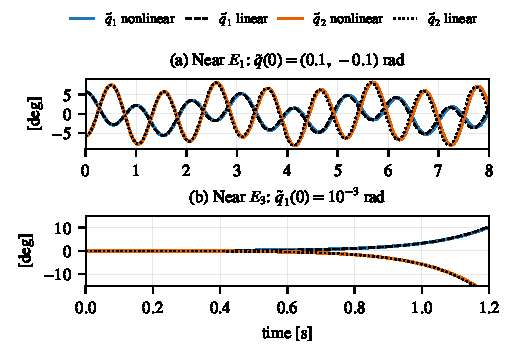
\includegraphics[width=0.55\textwidth]{figures/sim.pdf}
\caption{Nonlinear (colour) vs.\ linear (black) free responses near (a) $E_1$ and (b) $E_3$.}
\label{fig:sim}
\end{figure}
\subsection{Interactive Simulator}
The nonlinear model runs in PyBullet with an interactive dashboard (Fig.~\ref{fig:dash}). The user picks an equilibrium, an initial condition (slider, typed value or by dragging the arm) and a controller: open loop, single-angle PD, single-angle observer + LQR, full-state LQR, pole placement, elbow PD, or swing-up $\to$ LQR. The dashboard shows the nonlinear arm next to the linear model, $\tilde q(t)$, $\tau(t)$ and the closed-loop poles in the $s$-plane, all updating live. Files: \texttt{phase2/acrobot\_phase2\_sim.py}, \texttt{phase3/acrobot\_phase3\_sim.py}, \texttt{phase4/acrobot\_phase4\_sim.py} (instructions in each folder's \texttt{README.md}).
\begin{figure}[H]
\centering
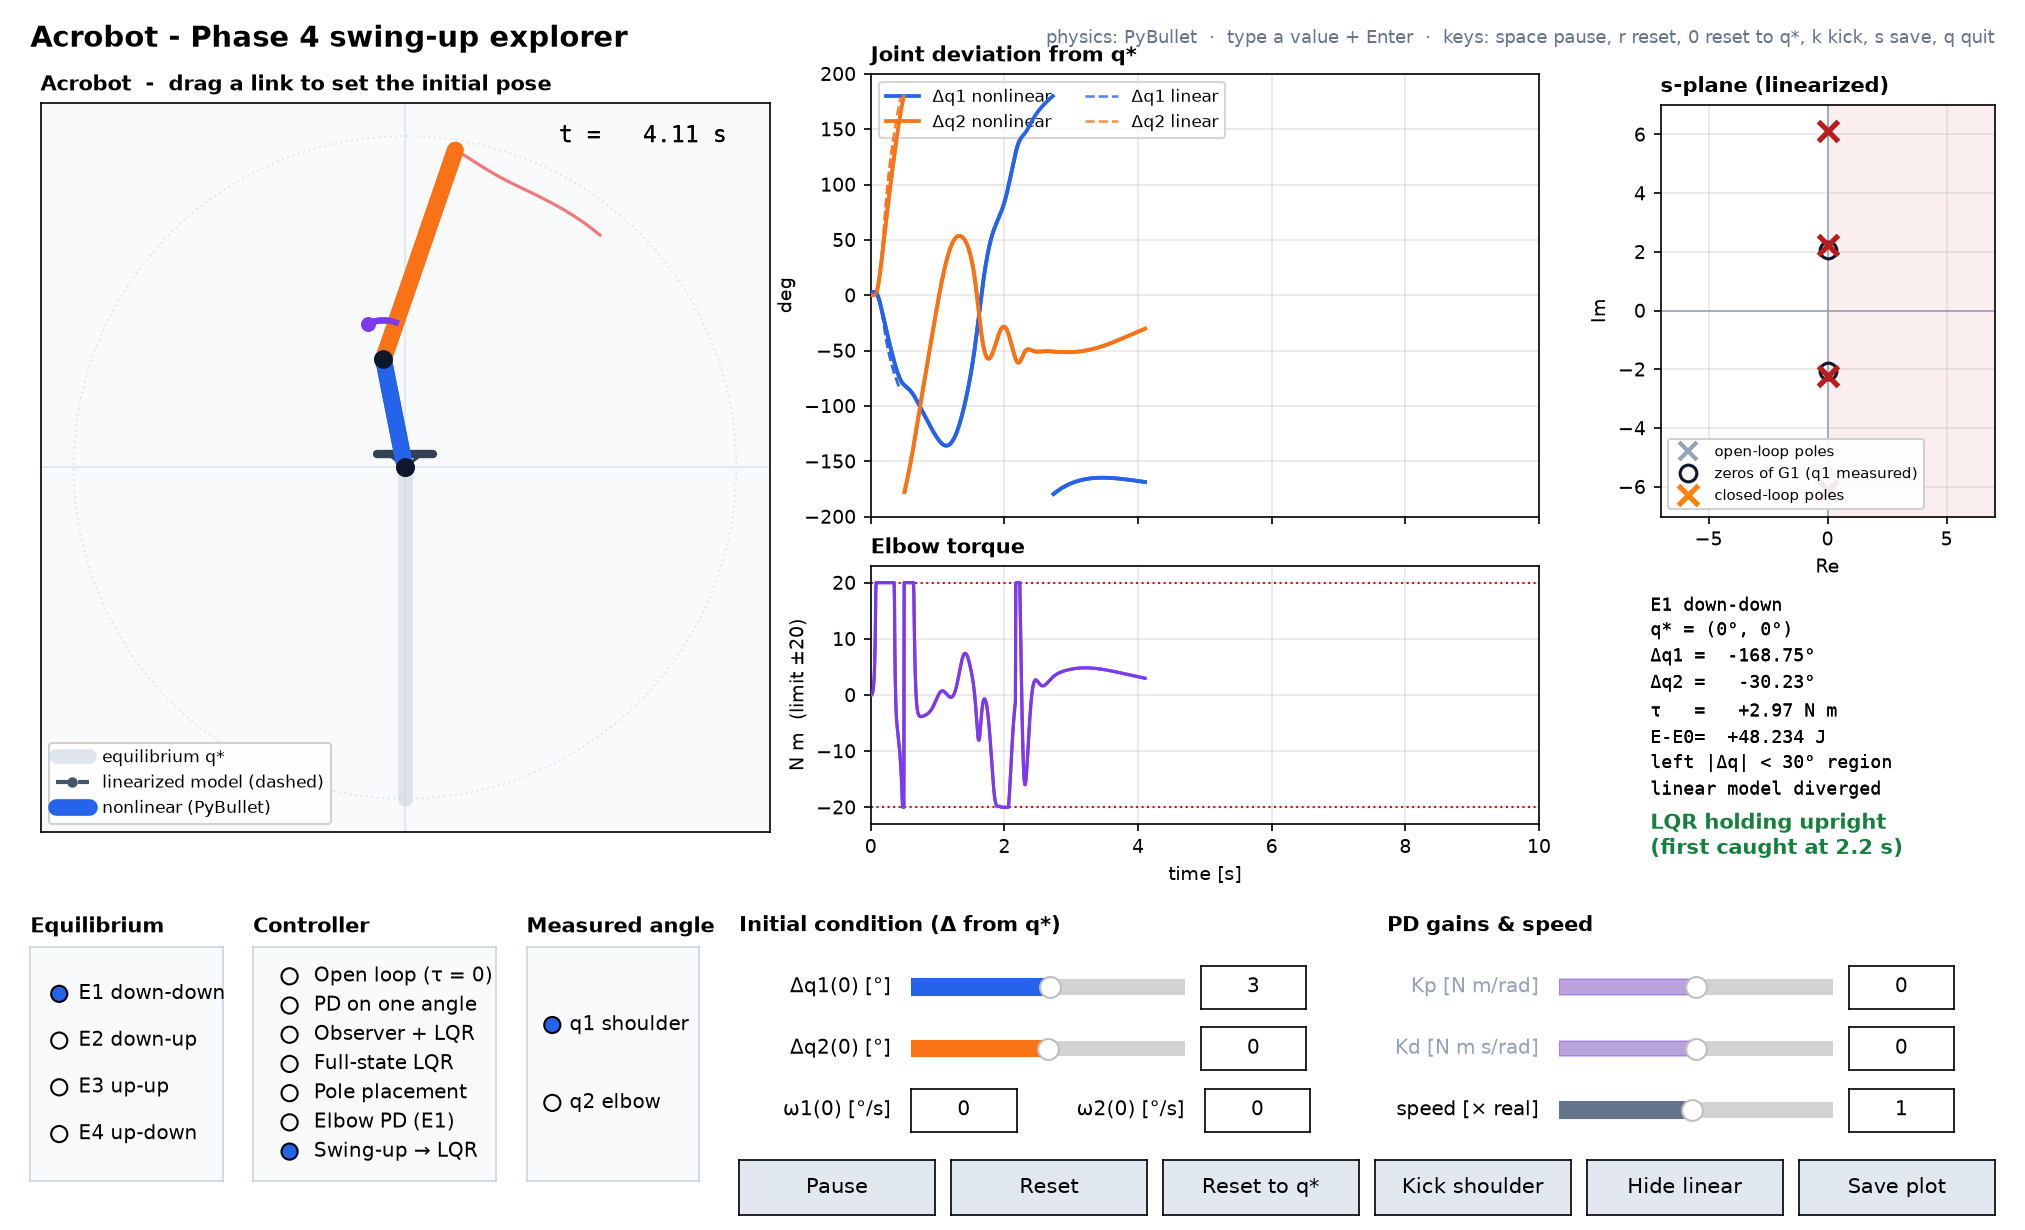
\includegraphics[width=\textwidth]{figures/dashboard.png}
\caption{Interactive PyBullet dashboard during a swing-up from hanging.}
\label{fig:dash}
\end{figure}


% =====================================================================
\section{Stability Analysis}\label{sec:stab}
% =====================================================================
\subsection{Stability Criteria}
\begin{itemize}
\item \textbf{State space:} the linear model~\eqref{eq:lin} is \emph{asymptotically stable} if every eigenvalue of $A$ has $\operatorname{Re}\lambda<0$, \emph{unstable} if any has $\operatorname{Re}\lambda>0$, and \emph{marginally stable} if the eigenvalues on the imaginary axis are simple and none lies to the right.
\item \textbf{Transfer function:} $G_j$ is \emph{BIBO stable} if every pole has $\operatorname{Re}p<0$.
\item \textbf{Nonlinear system (Lyapunov's indirect method):} an eigenvalue with $\operatorname{Re}\lambda>0$ makes the equilibrium of~\eqref{eq:eom} unstable; eigenvalues on the imaginary axis leave the question open [4].
\end{itemize}

\subsection{Poles of the Transfer Functions = Eigenvalues of $A$}
At every equilibrium
\[
\operatorname{rank}[B_\ell\ \ AB_\ell\ \ A^2B_\ell\ \ A^3B_\ell]=4,\qquad
\operatorname{rank}\begin{bmatrix}C_j\\C_jA\\C_jA^2\\C_jA^3\end{bmatrix}=4\quad(j=1,2),
\]
so both $G_1$ and $G_2$ are minimal realizations with no pole--zero cancellation. Their poles are exactly the eigenvalues of $A$, and the transfer-function and state-space verdicts must coincide.

\subsection{Characteristic Polynomial}
\begin{equation}
\Delta(s)=s^4+0\cdot s^3-\operatorname{tr}(P)\,s^2+0\cdot s+\det P .
\end{equation}
A Hurwitz polynomial has all coefficients positive. Here the $s^3$ and $s^1$ coefficients are zero because the model has no friction, so \textbf{no equilibrium is asymptotically stable with $\tau=0$}. Writing $\lambda=s^2$ (the eigenvalues of $P$):
\begin{equation}
\lambda^2-\operatorname{tr}(P)\lambda+\det P=0,\qquad \lambda<0\Rightarrow s=\pm j\sqrt{-\lambda},\qquad \lambda>0\Rightarrow s=\pm\sqrt\lambda .
\end{equation}
\begin{itemize}
\item $\det P>0$, $\operatorname{tr}P<0$: both $\lambda<0$, all poles on the $j\omega$-axis ($E_1$).
\item $\det P<0$: one $\lambda$ of each sign, one real RHP pole ($E_2$, $E_4$).
\item $\det P>0$, $\operatorname{tr}P>0$: both $\lambda>0$, two RHP poles ($E_3$).
\end{itemize}

\subsection{Link to the Potential Energy}
Since $K=-\nabla^2U$ and $M\succ0$, $P=M^{-1}K$ is similar to $M^{-1/2}KM^{-1/2}$, which is congruent to $K$. By Sylvester's law of inertia,
\begin{equation}
\#\{\text{RHP poles}\}=\#\{\text{negative eigenvalues of }\nabla^2U\}.
\end{equation}
A minimum of $U$ gives no RHP pole, a saddle one, and a maximum two [3].

\subsection{Stability of Each Equilibrium}
\begin{table}[H]
\centering
\caption{Stability of the four equilibria}
\label{tab:stab}
\small
\resizebox{\textwidth}{!}{\begin{tabular}{|c|c|c|c|c|c|}
\hline
 & $(\operatorname{tr}P,\det P)$ & poles of $G_1,G_2$ $=$ eig$(A)$ & eig$\nabla^2U$ & RHP & Verdict\\ \hline
$E_1$ & $(-42.24,\ 186.77)$ & $\pm j2.2400,\ \pm j6.1011$ & $4.91,\ 29.43$ (min) & 0 & marginally stable\\
$E_2$ & $(-8.40,\ -186.77)$ & $\pm3.1775,\ \pm j4.3010$ & $-14.72,\ 9.81$ (saddle) & 1 & unstable\\
$E_3$ & $(42.24,\ 186.77)$ & $\pm2.2400,\ \pm6.1011$ & $-29.43,\ -4.91$ (max) & 2 & unstable\\
$E_4$ & $(8.40,\ -186.77)$ & $\pm4.3010,\ \pm j3.1775$ & $-9.81,\ 14.72$ (saddle) & 1 & unstable\\ \hline
\end{tabular}}
\end{table}

\textbf{$E_1$ (down--down).}
\begin{itemize}
\item \textbf{Transfer function:} the poles are simple and on the imaginary axis, so $G_1$ and $G_2$ are \emph{not} BIBO stable. A bounded input at a resonance, $\tau=\sin(2.24t)$, gives a double pole at $\pm j2.24$ and a response that grows like $t\sin(2.24t)$.
\item \textbf{State space:} the free response is a sum of two undamped modes ($\omega=2.24$ and $6.10$~rad/s): bounded but not decaying, so \textbf{marginally stable}.
\item \textbf{Nonlinear:} linearization is inconclusive, so we use energy as a Lyapunov function:
\begin{equation}
V(x)=\tfrac12\dot q^TM(q)\dot q+U(q)-U(q^*),\qquad \nabla^2U(q^*)\succ0\Rightarrow V\succ0,\qquad \dot V=\dot q^TB\tau=0 .
\end{equation}
$E_1$ is \textbf{stable in the sense of Lyapunov but not asymptotically stable}: the swing never decays.
\end{itemize}

\textbf{$E_2$ and $E_4$ (one link up).} $\det P=-186.77<0$, so each has one real RHP pole ($+3.1775$ at $E_2$, $+4.3010$ at $E_4$). Both are BIBO unstable, $A$ is unstable, and by Lyapunov's indirect method the nonlinear equilibria are unstable.

\textbf{$E_3$ (up--up).} Gravity flips, $P_{E3}=-P_{E1}$, so $\lambda$ changes sign and the poles become $\pm2.2400$, $\pm6.1011$: \textbf{two RHP poles}, unstable in every sense.

\subsection{Simulation Evidence}
All simulations use the full nonlinear model in \textbf{PyBullet} [5] (uniform rods, no damping, step $0.25$~ms). Checked against an RK4 integration of~\eqref{eq:eom} with $q(0)=(0.8,-0.5)$~rad and $\tau=3\sin2t$, the two agree to within $0.52^\circ$ over 5~s.
\begin{figure}[H]
\centering
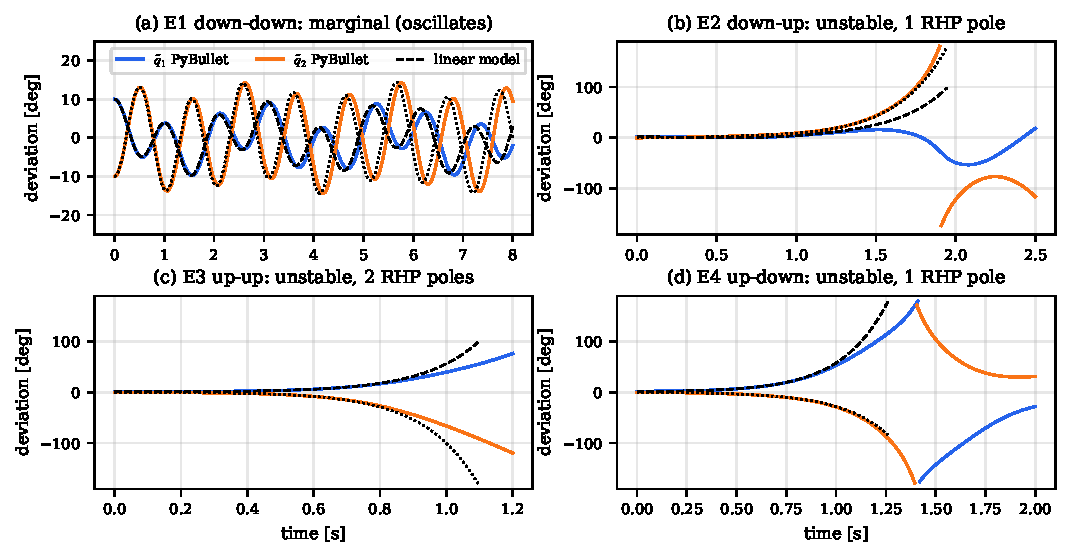
\includegraphics[width=\textwidth]{figures/fig_openloop.pdf}
\caption{Free response ($\tau=0$) near each equilibrium: PyBullet (colour) vs.\ linear model (black).}
\label{fig:ol}
\end{figure}
\begin{figure}[H]
\centering
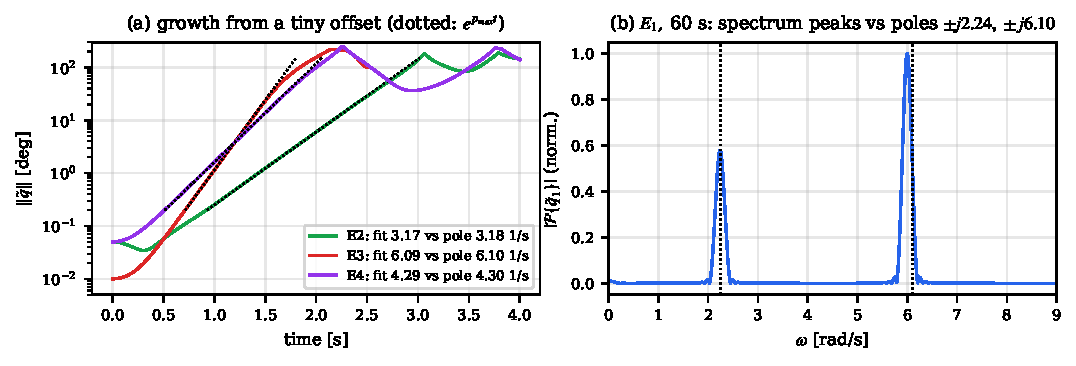
\includegraphics[width=\textwidth]{figures/fig_growth.pdf}
\caption{(a) Growth of a tiny offset on a log scale; dotted lines have the slope of the largest RHP pole. (b) Spectrum of $\tilde q_1$ near $E_1$; dotted lines are the poles.}
\label{fig:growth}
\end{figure}
\begin{table}[H]
\centering
\caption{Linear predictions vs.\ PyBullet measurements}
\label{tab:evidence}
\small
\begin{tabular}{|c|l|c|c|c|}
\hline
 & Quantity & Predicted & Measured & Error\\ \hline
$E_1$ & oscillation frequencies & $2.240,\ 6.101$ rad/s & $2.239,\ 5.997$ rad/s & within 1 bin\\
$E_1$ & energy change over 60 s & $0$ & $1.2\times10^{-3}$ J & integration error\\
$E_2$ & growth rate & $3.1775$ s$^{-1}$ & $3.171$ s$^{-1}$ & $0.22\%$\\
$E_3$ & growth rate & $6.1011$ s$^{-1}$ & $6.088$ s$^{-1}$ & $0.21\%$\\
$E_4$ & growth rate & $4.3010$ s$^{-1}$ & $4.294$ s$^{-1}$ & $0.15\%$\\ \hline
\end{tabular}
\end{table}
\textbf{Observations:}
\begin{itemize}
\item $E_1$ oscillates forever at its initial amplitude, with frequencies matching the poles.
\item A tiny offset at $E_2$, $E_3$, $E_4$ grows exponentially at exactly the rate of the largest RHP pole. At $E_3$ a $0.01^\circ$ tilt reaches $30^\circ$ in $1.55$~s.
\item The linear model tracks the nonlinear one until about $20^\circ$, then over-predicts.
\end{itemize}

% =====================================================================
\section{Feedback from a Single Measured Angle}\label{sec:single}
% =====================================================================

\subsection{Static or PD Feedback}
Measuring one angle $y=\tilde q_j$ and applying $\tau=-(K_p+K_ds)\,y$ with $G_j=(b_2s^2+b_0)/(s^4+a_2s^2+a_0)$ gives the closed-loop polynomial
\begin{equation}
s^4+(K_db_2)\,s^3+(a_2+K_pb_2)\,s^2+(K_db_0)\,s+(a_0+K_pb_0) .\label{eq:pd}
\end{equation}
Hurwitz requires $K_db_2>0$ \emph{and} $K_db_0>0$, i.e.\ $b_2$ and $b_0$ of the same sign. At $E_3$:
\begin{itemize}
\item measuring $q_1$: $b_2=-3.0147$, $b_0=+12.6926$, opposite signs;
\item measuring $q_2$: $b_2=+6.0332$, $b_0=-31.7316$, opposite signs.
\end{itemize}
The signs are opposite because the zeros $\pm2.0519$ and $\pm2.2934$ are \textbf{real}: one of each pair lies in the right half-plane. \textbf{No $K_p$, $K_d$ can stabilize $E_3$ from one angle.} A grid search confirms it: the smallest attainable largest real part is $0.96$ ($q_1$) and $2.29$ ($q_2$), and in PyBullet even these gains fall from $1^\circ$ within 2~s.
\begin{figure}[H]
\centering
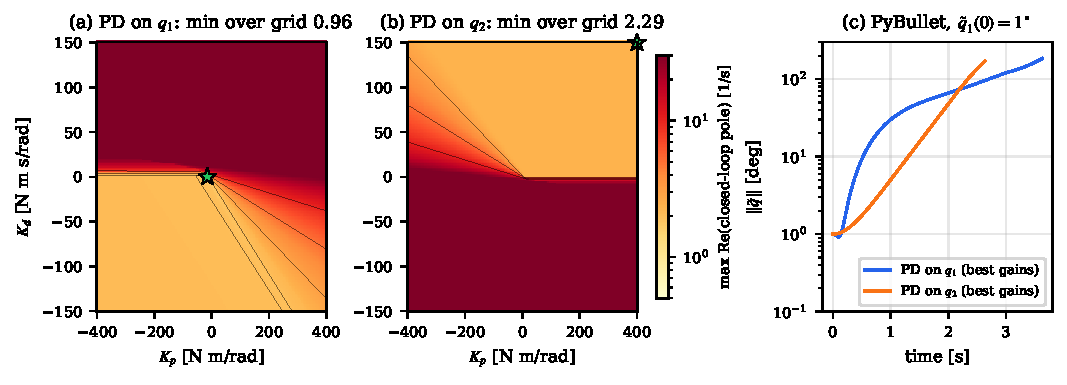
\includegraphics[width=\textwidth]{figures/fig_pd.pdf}
\caption{PD from one angle at $E_3$: (a, b) largest closed-loop real part over the gain plane, positive everywhere; (c) PyBullet with the best gains.}
\label{fig:pd}
\end{figure}

\subsection{Dynamic (Observer-Based) Feedback}
Each angle alone makes $(A,C_j)$ observable, so an observer can reconstruct the full state and LQR can act on the estimate:
\begin{equation}
\dot{\hat x}=A\hat x+B_\ell\tau+L(y-C_j\hat x),\qquad \tau=-K\hat x,\qquad \lambda_{cl}=\lambda(A-B_\ell K)\cup\lambda(A-LC_j).
\end{equation}
Two limits apply to \emph{any} controller:
\begin{itemize}
\item \textbf{Parity interlacing [6]:} for $q_1$ the interval $(2.05,\infty)$ contains two real RHP poles, so a stable controller suffices. For $q_2$, $(2.29,\infty)$ contains one, so the controller itself must be unstable.
\item \textbf{Sensitivity bound [3]:} $\|S\|_\infty\ge\prod_i|z+p_i|/|z-p_i|$, which is $\ge45.9$ for $q_1$ and $\ge187$ for $q_2$, because each zero sits just below the pole $2.24$.
\end{itemize}
In PyBullet the observer-based loop holds $E_3$ only from $1.42^\circ$ (measuring $q_1$) or $0.23^\circ$ (measuring $q_2$), against $4.64^\circ$ with full-state feedback.
\begin{figure}[H]
\centering
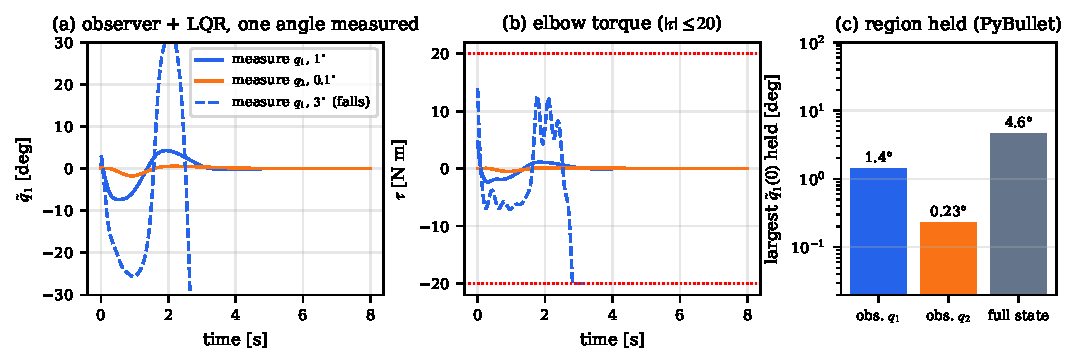
\includegraphics[width=\textwidth]{figures/fig_observer.pdf}
\caption{Observer + LQR at $E_3$ in PyBullet using one angle: (a) $\tilde q_1$; (b) torque; (c) largest initial offset held.}
\label{fig:obs}
\end{figure}
\textbf{Answer:} static or PD feedback from one joint angle \textbf{cannot} stabilize the upright, because of the real RHP zero. A dynamic controller \textbf{can}, but only for about a degree with $|\tau|\le20\Nm$, so full-state feedback is used from here on (Section~\ref{sec:ctrl}).

% =====================================================================
% =====================================================================
\section{Controller Design Around the Equilibria}\label{sec:ctrl}
% =====================================================================
\subsection{Controller Design}
The rank of $\mathcal C$ is 4 at every equilibrium, so all four states can be fed back. Including the torque limit, every controller has the form
\begin{equation}
\tau=\operatorname{sat}(-K\tilde x),\qquad \tilde x=[\tilde q_1,\ \tilde q_2,\ \dot q_1,\ \dot q_2]^T,\qquad |\tau|\le20\Nm .
\end{equation}
The controllers used are:
\begin{itemize}
\item \textbf{LQR} at the upright $E_3$, at $E_2$ and at $E_4$;
\item \textbf{pole placement} at $E_3$, for comparison;
\item \textbf{PD on the elbow angle only} at $E_1$.
\end{itemize}

\subsection{Linear Quadratic Regulator (LQR)}
$K$ minimizes a cost that penalizes both the state error and the torque:
\begin{equation}
J=\int_0^\infty\big(\tilde x^TQ\tilde x+R\,\tau^2\big)\,dt,\qquad A^TS+SA-SB_\ell R^{-1}B_\ell^TS+Q=0,\qquad K=R^{-1}B_\ell^TS .
\end{equation}
\textbf{Expected performance of LQR:}
\begin{itemize}
\item \textbf{Stability:} guaranteed for any $Q\succeq0$, $R>0$ when $(A,B_\ell)$ is controllable.
\item \textbf{Robustness:} phase margin $\ge60^\circ$ and gain margin $[\frac12,\infty)$ [7].
\item \textbf{Tuning:} $Q=I$ weighs 1~rad of angle like 1~rad/s of rate. A smaller $R$ makes the controller faster but demands more torque, so $R$ trades speed against saturation.
\end{itemize}

\subsubsection{Choice of $R$}
For each $R$ we simulated the nonlinear saturated loop from a grid of initial offsets and counted how many were recovered (Fig.~\ref{fig:design}).
\begin{itemize}
\item \textbf{$E_3$:} the recovered area stays at 16--20\% of a $\pm60^\circ$ grid for $10^{-3}\le R\le1$, while the fastest pole moves from $-10$ to $-214$~s$^{-1}$. The limit is $\tau_{\max}$, not the tuning. $R=0.03$ is the knee: 93\% of the best area with a fastest pole of $-40$.
\item \textbf{$E_2$:} the region collapses for $R>0.3$ ($99\%\to90\%\to20\%$), so $R=0.1$.
\item \textbf{$E_4$:} the area peaks at $R\approx0.1$--$0.18$, so $R=0.1$.
\end{itemize}
\begin{figure}[H]
\centering
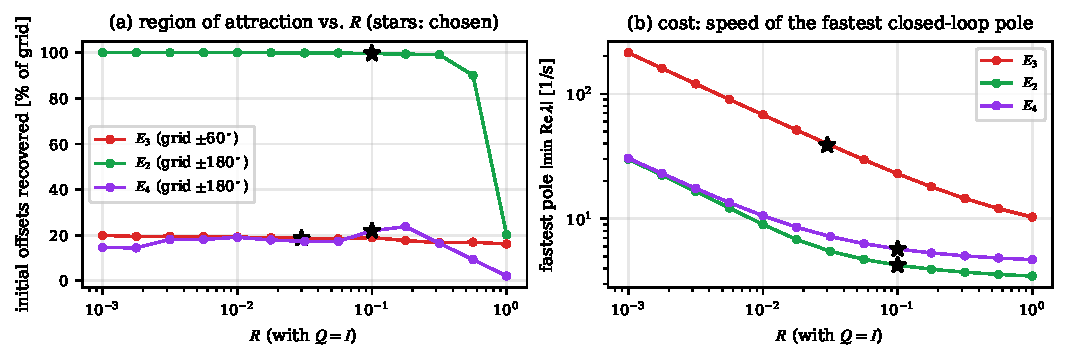
\includegraphics[width=\textwidth]{figures/fig_design.pdf}
\caption{Weight selection ($Q=I$): (a) share of offsets recovered; (b) fastest closed-loop pole. Stars: chosen $R$.}
\label{fig:design}
\end{figure}

\subsection{Pole Placement at $E_3$ (Comparison)}
Placing the poles at $\{-3,-4,-5,-6\}$ gives $K=[-322.9,\,-134.6,\,-138.1,\,-66.0]$. It settles faster from $2^\circ$ ($1.3$~s vs $4.1$~s) and with less torque ($11.3$ vs $17.6\Nm$), but recovers a smaller region ($20\%$ vs $26\%$ of $\pm40^\circ$; $5^\circ$ vs $6^\circ$ along $q_1$). LQR is therefore kept for $E_3$.

\subsection{$E_1$: PD on the Elbow Angle Only}
At $E_1$ the zeros of $G_2$ are imaginary ($\pm j2.29$), so the sign conflict of~\eqref{eq:pd} does not arise and one angle suffices:
\begin{equation}
\tau=-K_p\tilde q_2-K_d\dot q_2,\qquad K_p=-5,\quad K_d=0.4,
\end{equation}
the pair with the best decay rate on a $(K_p,K_d)$ grid ($\max\operatorname{Re}\lambda=-0.52$).
\textbf{Proof of stability (energy shaping, LaSalle [4]):}
\begin{gather}
V_c=E-E^*+\tfrac12K_p\tilde q_2^{\,2},\qquad \dot V_c=-K_d\,\dot q_2^{\,2}\le0,\\
\nabla^2\big(U+\tfrac12K_p\tilde q_2^{\,2}\big)\big|_{E_1}\ \text{has eigenvalues}\ 0.760,\ 28.575>0 .\nonumber
\end{gather}
$V_c$ has a strict minimum at $E_1$ and never increases, and $\dot q_2\equiv0$ only at $E_1$, so $E_1$ is asymptotically stable. Pure damping ($K_p=0$) decays $19\times$ more slowly.

\subsection{Designed Controllers}
\begin{table}[H]
\centering
\caption{Designed controllers and their closed-loop poles}
\label{tab:ctrl}
\small
\resizebox{\textwidth}{!}{\begin{tabular}{|l|l|l|l|}
\hline
Controller & Design & $K=[k_{q_1},k_{q_2},k_{\dot q_1},k_{\dot q_2}]$ & Closed-loop poles\\ \hline
$E_3$ LQR & $Q=I$, $R=0.03$ & $[-503.0,\,-203.9,\,-218.3,\,-101.5]$ & $-39.86,\,-2.25\pm0.10j,\,-1.34$\\
$E_3$ pole placement & $\{-3,-4,-5,-6\}$ & $[-322.9,\,-134.6,\,-138.1,\,-66.0]$ & $-6,\,-5,\,-4,\,-3$\\
$E_2$ LQR & $Q=I$, $R=0.1$ & $[6.60,\,46.49,\,5.23,\,13.24]$ & $-4.26,\,-2.40,\,-1.24\pm4.16j$\\
$E_4$ LQR & $Q=I$, $R=0.1$ & $[-49.31,\,38.91,\,-13.19,\,6.10]$ & $-5.73,\,-3.21,\,-0.96\pm3.08j$\\
$E_1$ elbow PD & $K_p=-5$, $K_d=0.4$ & $[0,\,-5,\,0,\,0.4]$ & $-0.69\pm2.31j,\,-0.52\pm2.14j$\\ \hline
\end{tabular}}
\end{table}

% =====================================================================
\section{Performance Limits under the Torque Limit}\label{sec:limits}
% =====================================================================

\subsection{Guaranteed Region}
Inside $\Omega_c=\{\tilde x^TS\tilde x\le c\}$ the command never saturates if
\begin{equation}
c^*=\frac{\tau_{\max}^2}{KS^{-1}K^T},\qquad \dot V=-\tilde x^T(Q+K^TRK)\tilde x<0\ \text{ on }\Omega_{c^*}.
\end{equation}
At rest this guarantees $0.72^\circ/1.66^\circ$ ($E_3$), $45.6^\circ/19.9^\circ$ ($E_2$) and $20.0^\circ/23.1^\circ$ ($E_4$) along $q_1$/$q_2$. The bound is conservative because short saturation is usually survived.

\subsection{Simulated Region of Attraction}
The real limits come from simulating the nonlinear saturated loop from a grid of initial offsets at rest. A start counts as recovered if it ends within $1^\circ$ and $0.05$~rad/s of $q^*$. The fast integrator used for the grids matches PyBullet on 100\% of random points and 96\% of boundary points.
\begin{figure}[H]
\centering
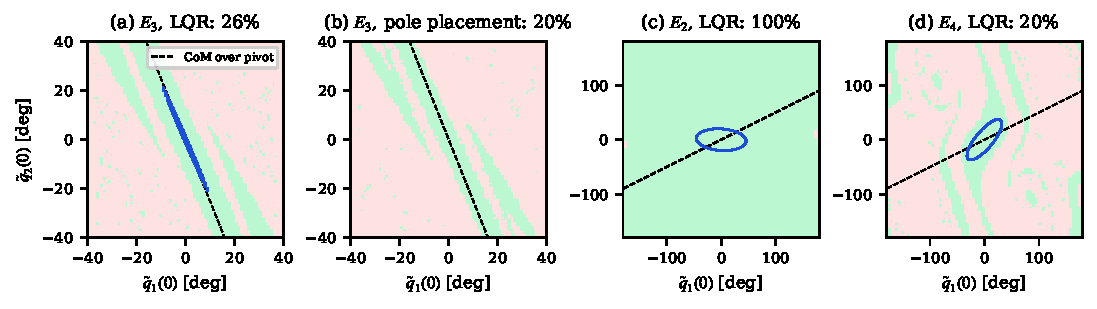
\includegraphics[width=\textwidth]{figures/fig_roa.pdf}
\caption{Region of attraction (green: recovered). Blue ellipse: guaranteed region. Dashed: offsets with the centre of mass over the pivot.}
\label{fig:roa}
\end{figure}
\begin{table}[H]
\centering
\caption{How far from the equilibrium each controller still works}
\label{tab:limits}
\small
\resizebox{\textwidth}{!}{\begin{tabular}{|l|c|c|c|c|c|}
\hline
Controller & Recovered (grid) & $|\tilde q_1(0)|$ alone & $|\tilde q_2(0)|$ alone & Shoulder kick & Settling\\ \hline
$E_3$ LQR & 26\% ($\pm40^\circ$) & $6^\circ$ & $13^\circ$ & $0.20$ rad/s & $4.1$ s\\
$E_3$ pole placement & 20\% ($\pm40^\circ$) & $5^\circ$ & $9^\circ$ & $0.15$ rad/s & $1.3$ s\\
$E_2$ LQR & 99.7\% ($\pm180^\circ$) & $175^\circ$ & $180^\circ$ & $\ge8$ rad/s & $3.0$ s\\
$E_4$ LQR & 20.5\% ($\pm180^\circ$) & $35^\circ$ & $55^\circ$ & $2.1$ rad/s & $3.6$ s\\
$E_1$ elbow PD & 77.8\% ($\pm180^\circ$) & $40^\circ$ & $115^\circ$ & $2.15$ rad/s & $12.8$ s\\ \hline
\end{tabular}}
\end{table}

\textbf{Why the upright region is a thin band.} Linearizing $\tau_g$ at $E_3$:
\begin{equation}
\tau_{g,1}=9.81\,(2.5\,\tilde q_1+\tilde q_2).
\end{equation}
Gravity pushes the passive shoulder in proportion to the horizontal offset of the total centre of mass. The motor can only counter this through the elbow coupling. Along $\tilde q_2=-2.5\,\tilde q_1$ there is no shoulder torque, and the region reaches the grid edge ($\ge43^\circ$). Across that line, $20\Nm$ is used up after about $6^\circ$.

\subsection{Time Responses}
\begin{figure}[H]
\centering
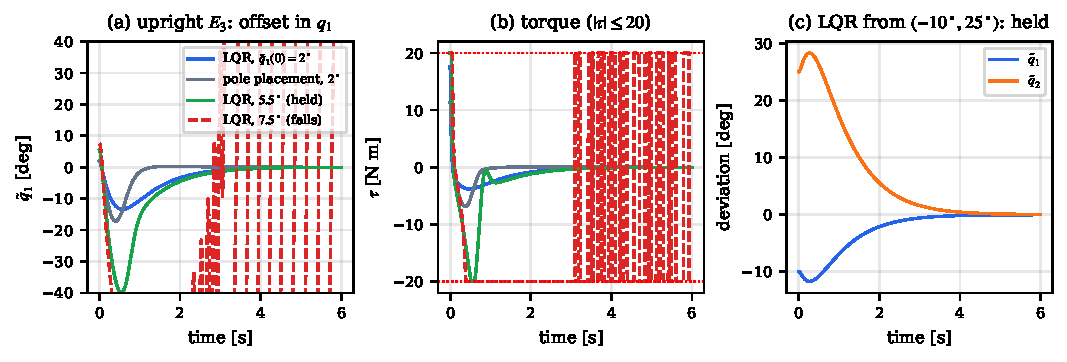
\includegraphics[width=\textwidth]{figures/fig_e3.pdf}
\caption{$E_3$ in PyBullet: LQR is held from $5.5^\circ$ and falls from $7.5^\circ$; a CoM-balanced offset $(-10^\circ,25^\circ)$ is held with only $3.3\Nm$.}
\label{fig:e3}
\end{figure}
\begin{figure}[H]
\centering
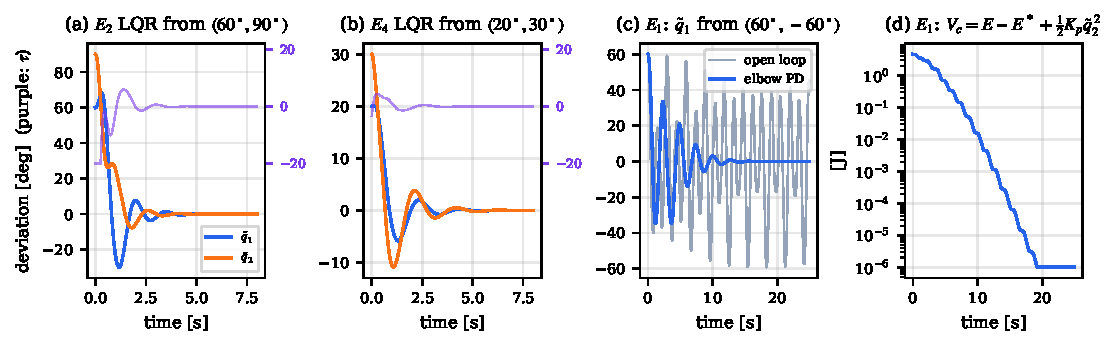
\includegraphics[width=\textwidth]{figures/fig_others.pdf}
\caption{(a) $E_2$ and (b) $E_4$ with LQR; (c) $E_1$ with elbow PD vs.\ open loop; (d) $V_c$ decreasing along the $E_1$ run.}
\label{fig:others}
\end{figure}
\textbf{Observations:}
\begin{itemize}
\item \textbf{Settling time:} pole placement settles fastest at $E_3$, but LQR rescues a larger region. $E_1$ is slowest ($12.8$~s) because its slow mode barely moves the elbow.
\item \textbf{Control effort:} at $E_3$ even a $2^\circ$ offset needs $17.6\Nm$, close to the limit, which explains the small region. At $E_4$ the peak is only $4.5\Nm$.
\item \textbf{Steady-state error:} zero for every controller (each converges to $q^*$ within $0.001^\circ$).
\end{itemize}

% =====================================================================
% =====================================================================
\section{Swing-Up Control}\label{sec:swing}
% =====================================================================
\subsection{Energy Target}
Hanging has $E=U(E_1)=-24.525$~J and the upright needs $E_{top}=U(E_3)=+24.525$~J. The controller must therefore add $49$~J with a $20\Nm$ elbow motor, and deliver the arm close enough to $E_3$ for the upright LQR of Section~\ref{sec:ctrl} to catch it.

\subsection{Swing-Up Controller}
\textbf{Partial feedback linearization.} With $h=C\dot q-\tau_g$, row~1 of~\eqref{eq:eom} gives $\ddot q_1=-(M_{12}\ddot q_2+h_1)/M_{11}$. Substituting into row~2, the elbow follows any desired acceleration $v$ exactly:
\begin{equation}
\tau=\Big(M_{22}-\frac{M_{21}M_{12}}{M_{11}}\Big)v+h_2-\frac{M_{21}h_1}{M_{11}}\ \Rightarrow\ \ddot q_2=v .
\end{equation}
\textbf{Energy pumping.} The desired elbow acceleration is
\begin{equation}
v=-k_1\tilde q_2-k_2\dot q_2+k_3\,\dot q_1\,(E-E_{top}) .\label{eq:v}
\end{equation}
\begin{itemize}
\item $k_1$, $k_2$: keep the elbow nearly straight (a stiff and damped elbow).
\item $k_3$: pushes in step with $\dot q_1$ while $E<E_{top}$ (adds energy) and against it when $E>E_{top}$ (removes energy), like a child pumping a swing.
\end{itemize}

\subsection{Hybrid Switching}
\begin{equation}
\tau=\operatorname{sat}\begin{cases}-K\tilde x, & \tilde x^TS\tilde x<c_{sw}=5\quad\text{(catch: LQR at $E_3$, Sec.~\ref{sec:ctrl})}\\ \text{swing-up law above}, & \text{otherwise}\end{cases}
\end{equation}
If the arm leaves the catch region (a missed catch or a push), swing-up resumes automatically.

\subsection{Choice of Gains}
We searched 144 designs ($k_1\in\{20,50,100\}$, $k_2\in\{2,5,10\}$, $k_3\in\{0.3,1,3,10\}$, $c_{sw}\in\{0.5,1,2,5\}$) from $0.05$~rad off hanging; 22 swung up and held. Each was then rerun from 40 random starts. \textbf{$k=(20,2,3)$, $c_{sw}=5$} succeeded from \textbf{39/40}, with a median first catch of $4.0$~s.

\subsection{Results}
\begin{table}[H]
\centering
\caption{Swing-up runs in PyBullet ($|\tau|\le20\Nm$)}
\label{tab:swing}
\small
\resizebox{\textwidth}{!}{\begin{tabular}{|l|c|c|c|c|}
\hline
Start (from hanging) & First catch & Final deviation from $E_3$ & Torque saturated & Result\\ \hline
$(3^\circ,0)$, $k=(20,2,3)$ & $2.2$ s & $<0.001^\circ$ & 5\% & held\\
$(-10^\circ,20^\circ)$, $k=(20,2,3)$ & $9.5$ s & $<0.01^\circ$ & 17\% & held\\
$(3^\circ,0)$, kick $0.8$ rad/s at 8 s & $2.2$ s, re-caught & $<0.001^\circ$ & 5\% & held\\
$(3^\circ,0)$, textbook $k=(50,5,10)$ & $8.4$ s & $<0.001^\circ$ & 7\% & held (this start)\\ \hline
\end{tabular}}
\end{table}
\begin{figure}[H]
\centering
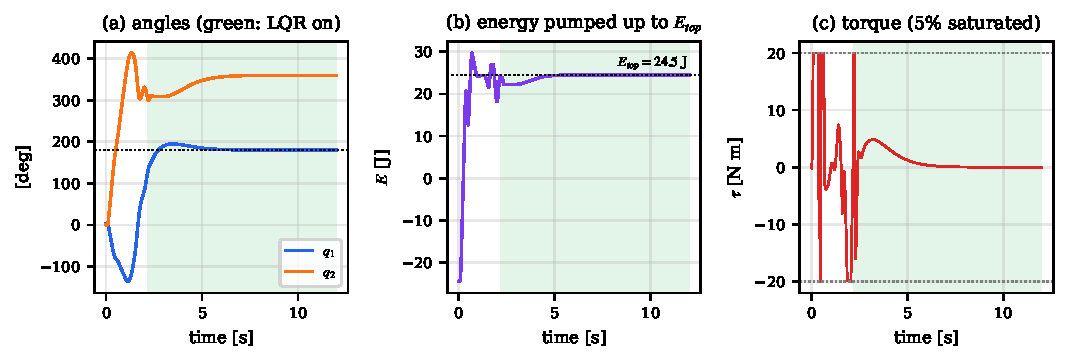
\includegraphics[width=\textwidth]{figures/fig_swingup.pdf}
\caption{Swing-up from $3^\circ$: (a) angles, (b) energy pumped to $E_{top}$, (c) torque. Green: LQR active.}
\label{fig:swingup}
\end{figure}

\subsection{Why It Works, and Why Other Gains Fail}
\begin{table}[H]
\centering
\caption{Success from 40 random starts vs.\ saturation during swing-up}
\label{tab:sat}
\begin{tabular}{|l|c|c|}
\hline
Gains $(k_1,k_2,k_3)$, $c_{sw}$ & Swing-up time at $|\tau|=20$ & Held (of 40)\\ \hline
$(20,2,3)$, 5 (chosen) & 26\% & \textbf{39}\\
$(50,2,3)$, 5 & 38\% & 4\\
$(100,2,3)$, 5 & 45\% & 2\\
$(20,2,0.3)$, 5 & 25\% & 0\\
$(50,5,10)$, 5 (textbook) & 33\% & 25\\
$(50,5,10)$, 1 (textbook) & 31\% & 13\\ \hline
\end{tabular}
\end{table}
\begin{enumerate}
\item \textbf{Saturation breaks the swing-up law.} The law assumes the full linearizing torque is applied. A stiff elbow (large $k_1$) asks for more than $20\Nm$ more often (26\% $\to$ 45\% of the time). While saturated $\ddot q_2\ne v$, the energy is no longer steered precisely, and the arm reaches the top off the catch region. Success drops from 39 to 2.
\item \textbf{Too little pumping.} With $k_3=0.3$ the energy approaches $E_{top}$ too slowly to reach the catch region within 40~s (0/40).
\item \textbf{The catch is the LQR limit.} The LQR recovers only a thin region around $E_3$. The swing-up only has to deliver the arm into that region, and $c_{sw}=5$ was the most reliable threshold tried.
\item \textbf{Retry.} Because swing-up resumes whenever $\tilde x^TS\tilde x\ge c_{sw}$, a missed catch or a push costs time, not the task (Fig.~\ref{fig:kick}a).
\end{enumerate}
\begin{figure}[H]
\centering
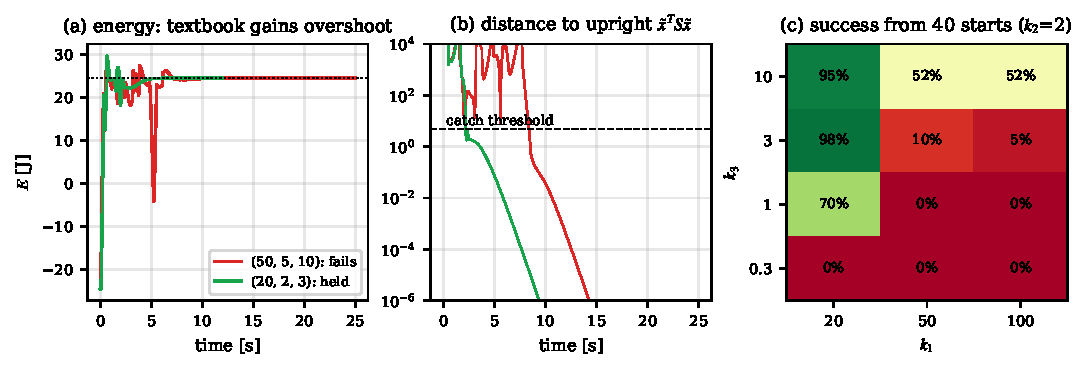
\includegraphics[width=\textwidth]{figures/fig_why.pdf}
\caption{(a) Energy, chosen vs.\ textbook gains; (b) distance to the upright and the catch threshold; (c) success rate over $(k_1,k_3)$.}
\label{fig:why}
\end{figure}
\begin{figure}[H]
\centering
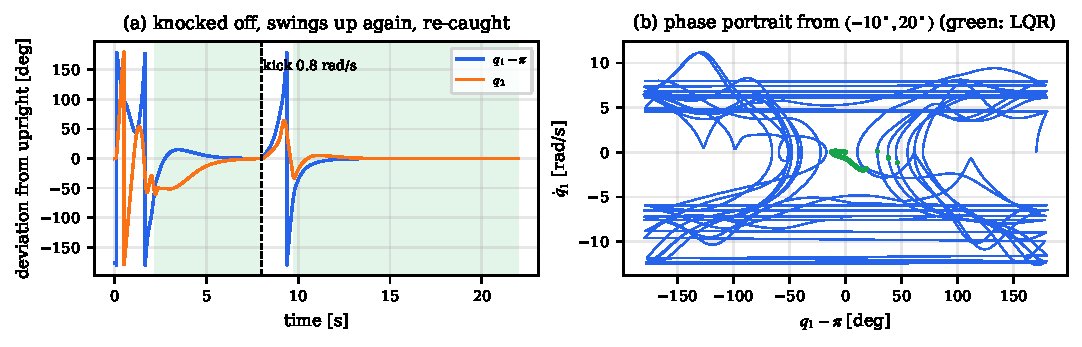
\includegraphics[width=0.9\textwidth]{figures/fig_kick.pdf}
\caption{(a) Knocked off at 8~s, swung up and caught again; (b) phase portrait from $(-10^\circ,20^\circ)$, green where LQR is active.}
\label{fig:kick}
\end{figure}

% =====================================================================
% =====================================================================
\section{Learning-Based Swing-Up}\label{sec:rl}
% =====================================================================

% =====================================================================
\subsection{Why Reinforcement Learning?}
The energy swing-up of Section~\ref{sec:swing} works, but it is built entirely from the model: the partial feedback linearization needs $M(q)$, $C(q,\dot q)$ and $\tau_g(q)$, and the energy target needs the exact masses and lengths. Reinforcement learning (RL) takes a different route. A neural-network policy learns \emph{by trial and error in a simulator} which torque to apply, guided only by a score (the reward). No equation of motion is written into the controller.
\begin{itemize}
\item \textbf{Question:} can a learned swing-up match or beat the hand-designed one under the same $20\Nm$ limit?
\item \textbf{Fair comparison:} both controllers hand over to the \emph{same} upright LQR of Section~\ref{sec:ctrl} inside the \emph{same} catch zone, so the only difference is who does the swing-up.
\item \textbf{Extra test:} what happens when the real robot differs from the model both controllers were designed or trained on?
\end{itemize}

\subsection{Hybrid Structure}
\begin{equation}
\tau=\begin{cases}\operatorname{sat}\big(-K\tilde x\big), & \tilde x^TS\tilde x<c_{sw}=5\quad\text{(catch: LQR, } R=0.03\text{, Sec.~\ref{sec:ctrl})}\\[2pt] 20\,\pi_\theta(o),\ \ \pi_\theta(o)\in[-1,1], & \text{otherwise (learned swing-up, held for 20 ms)}\end{cases}
\end{equation}
RL only has to deliver the arm into the catch zone; it never has to learn to balance. The part we can prove (the LQR near the top) stays model-based, and the hard nonlinear part is learned. If the arm leaves the zone, control returns to the policy, the same retry logic as the energy swing-up.

\subsection{Environment}
The environment follows the Gymnasium interface and uses the given equations of motion~\eqref{eq:eom}, integrated with RK4.
\begin{table}[H]
\centering
\caption{RL environment}
\label{tab:env}
\resizebox{\textwidth}{!}{\begin{tabular}{|l|l|l|}
\hline
Element & Choice & Reason\\ \hline
Observation $o$ & $[\cos q_1,\ \sin q_1,\ \cos q_2,\ \sin q_2,\ \dot q_1/10,\ \dot q_2/10]$ & no jump at $\pm180^\circ$; inputs of order 1\\
Action $a$ & $a\in[-1,1]$, $\tau=20\,a$ & the torque limit is built in: the policy cannot exceed it\\
Control step & 20 ms (50 Hz), four RK4 steps of 5 ms & realistic control rate\\
Start & $|\tilde q_i(0)|\le0.6$ rad, $|\dot q_i(0)|\le0.5$ rad/s around hanging & same spread as the robustness test of Section~\ref{sec:swing}\\
Episode & 15 s; ends early on entering the catch zone & short episodes, one clear goal\\ \hline
\end{tabular}}
\end{table}

\subsection{Reward Design}
\begin{multline}
r=-\Big(\frac{E-E_{top}}{E_{top}}\Big)^2-0.3\,(1+\cos q_1)-0.1\,(1-\cos q_2)\\
-0.001\Big(\frac{\tau}{20}\Big)^2+100\cdot\mathbb 1[\text{enter catch zone}] .
\end{multline}
\begin{itemize}
\item \textbf{Energy term:} the same target as the energy swing-up. It tells the policy \emph{how much} energy to pump. Without it, RL tends to learn to spin the arm round and round, because a spinning arm passes near the top often.
\item \textbf{Angle terms:} $1+\cos q_1$ is 0 when link~1 points up; $1-\cos q_2$ is 0 when the elbow is straight. They tell the policy \emph{where} to go.
\item \textbf{Torque term:} a small penalty that discourages wasted effort and bang--bang control.
\item \textbf{Catch bonus:} $+100$ for reaching the region where the LQR takes over; the episode then ends.
\end{itemize}

\subsection{Algorithm: Soft Actor-Critic (SAC)}
SAC [8] learns a stochastic policy $\pi_\theta$ (the actor) and two action-value networks $Q_\phi$ (the critics) that maximize reward plus entropy:
\begin{equation}
J(\pi)=\mathbb E\Big[\sum_t\gamma^t\big(r_t+\alpha\,\mathcal H(\pi(\cdot\mid o_t))\big)\Big].
\end{equation}
The entropy term $\mathcal H$ keeps the policy exploring, and $\alpha$ is tuned automatically. SAC suits this problem because the torque is continuous and SAC reuses past experience (off-policy), so it needs relatively few simulated swings.
\begin{table}[H]
\centering
\caption{Training settings (stable-baselines3 [9])}
\resizebox{\textwidth}{!}{\begin{tabular}{|l|l|}
\hline
Setting & Value\\ \hline
Networks & 2 hidden layers $\times$ 256 units (actor and critics)\\
Discount $\gamma$, learning rate, batch & $0.99$, $3\times10^{-4}$, 256\\
Replay buffer & 300\,000 transitions\\
Parallel environments, seed & 4, 0\\
Training length & $10^6$ steps $=$ 9\,206 episodes, 12.4 min on a laptop CPU\\ \hline
\end{tabular}}
\end{table}

\subsection{Training}
\begin{figure}[H]
\centering
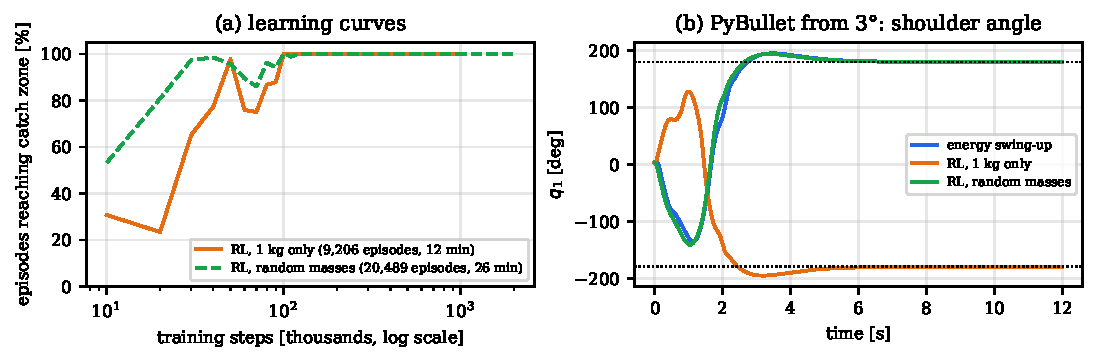
\includegraphics[width=\textwidth]{figures/fig_training.pdf}
\caption{(a) Share of training episodes that reached the catch zone, for the original policy and for the robust policy of Section~\ref{sec:robust} (log scale). (b) PyBullet runs from $3^\circ$: the original RL policy swings the other way and ends at $q_1=-180^\circ$, the same upright pose as $+180^\circ$; the robust policy swings the same way as the energy law.}
\label{fig:training}
\end{figure}
\textbf{Observations:}
\begin{itemize}
\item The policy first reached the catch zone in every episode after about $10^5$ steps (72~s of training) and stayed at 100\% for the remaining $9\times10^5$ steps.
\item Episodes kept getting shorter (more episodes per $10^4$ steps: 54 at $10^5$, 110 at $10^6$): the policy kept learning to reach the top faster.
\item The robust policy (Section~\ref{sec:robust}), which faces a different robot in every episode, also first reached 100\% after about $10^5$ steps. Over its remaining $1.9\times10^6$ steps it never dropped below 98.8\%.
\end{itemize}

\subsection{Results: Correct Model}
Both controllers were tested from the same 40 random starts as in Section~\ref{sec:swing}. A start counts as held if it is caught and balanced within 30~s. (This is why the energy controller scores 35 rather than the value of 39 in Section~\ref{sec:swing}, which allowed 40~s.)
\begin{table}[H]
\centering
\caption{RL vs.\ energy swing-up, correct masses ($|\tau|\le20\Nm$)}
\label{tab:rlnom}
\begin{tabular}{|l|c|c|}
\hline
Metric & Energy swing-up & RL swing-up (SAC)\\ \hline
Held (of 40) & 35 & \textbf{40}\\
Median time to first catch & 3.98 s & \textbf{1.71 s}\\
Time at the torque limit & 8.8\% & \textbf{0.1\%}\\
Median elbow work & 244.9 J & \textbf{144.5 J}\\
PyBullet from $3^\circ$: first catch & 2.17 s & \textbf{1.76 s}\\ \hline
\end{tabular}
\end{table}
\textbf{Observations:}
\begin{itemize}
\item \textbf{Reliability:} RL caught all 40 starts; the energy law caught 35 within 30~s.
\item \textbf{Speed:} RL reaches the top more than twice as fast (median 1.71 s vs.\ 3.98 s).
\item \textbf{Control effort:} RL almost never saturates the motor (0.1\% vs.\ 8.8\%) and uses 41\% less work. Saturation was what broke the energy law (Section~\ref{sec:swing}); the policy learned a timing that stays within $20\Nm$ by itself.
\end{itemize}

\subsection{Results: Wrong Model}
The real robot never matches the model exactly. The same 40 starts were rerun with both link masses changed by $\pm20\%$ (inertias scaled with them). Both controllers still assume 1~kg links.
\begin{table}[H]
\centering
\caption{Robustness to the link masses (held of 40, within 30 s)}
\label{tab:rlrob}
\begin{tabular}{|l|c|c|}
\hline
Link masses & Energy swing-up & RL swing-up (SAC)\\ \hline
$-20\%$ (0.8 kg) & 37 & 38\\
correct (1.0 kg) & 35 & 40\\
$+20\%$ (1.2 kg) & \textbf{35} & \textbf{15}\\ \hline
\end{tabular}
\end{table}
\begin{itemize}
\item \textbf{The energy law degrades gracefully} (35--37 of 40 in every case). It is built from physics: it pumps until $E=E_{top}$, so a heavier arm just takes a little longer (median 5.4~s instead of 4.0~s).
\item \textbf{RL collapses on heavier links} (15 of 40). It practised only on 1~kg links, so it learned the \emph{timing of that particular robot}, not the physics. It still reaches the catch zone in all 40 runs, but in a state from which the LQR cannot hold the heavier arm; it then repeats nearly the same approach (a median of 13 hand-overs in 30~s instead of 2).
\item \textbf{The fix} is to let the policy practise on many different robots (Section~\ref{sec:robust}).
\end{itemize}

\subsection{Making the Policy Robust}\label{sec:robust}
A second policy was trained with exactly \textbf{two changes}. Everything else (network, reward, catch zone, LQR and SAC settings) is the same, so any difference in the results comes from these two changes.
\begin{table}[H]
\centering
\caption{The two changes for the robust policy}
\label{tab:robustchanges}
\small
\begin{tabular}{|>{\raggedright\arraybackslash}p{2.5cm}|>{\raggedright\arraybackslash}p{3.0cm}|>{\raggedright\arraybackslash}p{4.6cm}|>{\raggedright\arraybackslash}p{4.0cm}|}
\hline
& \textbf{Original policy} & \textbf{Robust policy} & \textbf{Why}\\ \hline
1. Link masses in training & always 1 kg & new random $m_1,m_2\in[0.7,1.3]$ kg in every episode & it cannot memorise one robot's timing\\ \hline
2. Observation & the 6 numbers of Table~\ref{tab:env} & the same 6, plus the missing energy $(E_{top}-E)/E_{top}$ & the quantity the energy law steers by\\ \hline
Training length & $10^6$ steps, 9\,206 episodes, 12.4 min & $2\times10^6$ steps, 20\,489 episodes, 25.9 min & many robots make a harder task\\ \hline
\end{tabular}
\end{table}
The extra input is computed from the other six with the nominal 1~kg model, exactly as the energy controller computes it. It therefore adds no new information: it is a hint that makes the important quantity explicit. Change~1 is the real fix (this is called \emph{domain randomization}). By the end of training the robust policy reached the catch zone in 100\% of episodes, as the original did.

All three swing-ups were then tested from the same 40 starts with five link masses. Two of them (0.6 and 1.4 kg) lie \emph{outside} the range the robust policy practised on. Every controller still assumes 1~kg links.
\begin{table}[H]
\centering
\caption{Held of 40 random starts (within 30 s) for five link masses}
\label{tab:rlrob2}
\resizebox{\textwidth}{!}{\begin{tabular}{|l|c|c|c|}
\hline
True link masses & Energy swing-up & RL, 1 kg only & RL, random masses\\ \hline
0.6 kg ($-40\%$, never practised) & 39 & 2 & \textbf{40}\\
0.8 kg ($-20\%$) & 37 & 38 & \textbf{40}\\
1.0 kg (correct) & 35 & \textbf{40} & \textbf{40}\\
1.2 kg ($+20\%$) & 35 & 15 & \textbf{40}\\
1.4 kg ($+40\%$, never practised) & \textbf{33} & 3 & 2\\ \hline
\end{tabular}}
\end{table}
\begin{figure}[H]
\centering
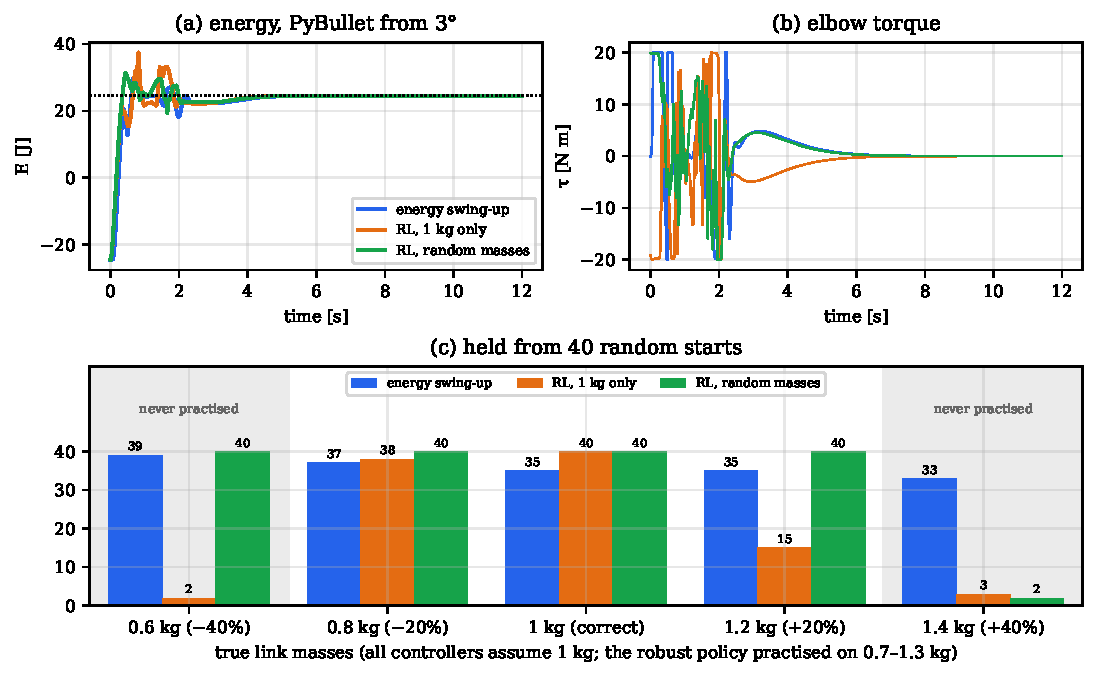
\includegraphics[width=\textwidth]{figures/fig_compare.pdf}
\caption{(a) Energy and (b) elbow torque in PyBullet from $3^\circ$ for the three swing-ups; (c) starts held for five link masses. Shaded: masses the robust policy never practised on.}
\label{fig:compare}
\end{figure}
\textbf{Observations:}
\begin{itemize}
\item \textbf{Inside the practised range the problem is solved:} 40 of 40 at every mass from 0.8 to 1.2~kg. At $+20\%$ the score rises from 15 to 40.
\item \textbf{No price on the correct model:} the robust policy also holds 40 of 40, with the same median catch time (1.71~s), no saturation (0.0\%) and 10\% less elbow work (130.0~J vs.\ 144.5~J). In PyBullet from $3^\circ$ it catches at 1.89~s (original 1.76~s).
\item \textbf{Lighter than ever practised (0.6~kg):} still 40 of 40. The original policy managed only 2, and in 25 of its 40 runs it never even reached the catch zone.
\item \textbf{Much heavier than ever practised (1.4~kg):} only 2 of 40, while the energy law still holds 33. The policy reaches the catch zone in all 40 runs, but the hand-over fails again and again (a median of 12 hand-overs in 30~s, against 1 for the energy law). The energy law also loses many first catches, but each new approach is different, so a later catch usually works; the policy repeats nearly the same approach.
\item \textbf{Why the hand-over is the weak point:} the reward ends the episode as soon as the arm \emph{enters} the catch zone. The policy is never told whether the LQR then holds the arm, so it never learned to deliver the arm in an easy-to-catch state.
\end{itemize}
\textbf{Lesson:} a learned controller is reliable over the variety of robots it practised on (here, also somewhat beyond it on the light side). A physics-based law knows \emph{why} it works, so it extrapolates further. Two natural next steps would be to reward holding rather than only arriving (end each episode only after the LQR has held the arm for, say, 1~s) and to widen the mass range.

\subsection{Discussion}
\begin{enumerate}
\item \textbf{Why RL is faster and gentler.} The energy law fixes the elbow motion through $v$ and pays for it with saturation. The policy is free to choose any torque profile and is rewarded for reaching the top quickly with little effort, so it found a timing that pumps energy faster without hitting the limit.
\item \textbf{Why RL was fragile, and what fixed it.} Its knowledge is implicit in $256\times256$ hidden units fitted to the robots it practised on. Practising on one robot gave that robot's timing; practising on many made it robust over that range. Nothing in it says ``pump until $E=E_{top}$'', however, so far outside that range (1.4~kg) it can still fail where the energy law does not.
\item \textbf{Guarantees.} The LQR catch has a Lyapunov certificate (Section~\ref{sec:limits}). The learned part has none: its performance is known only from tests, which is why it was tested on 40 starts, in a second simulator (PyBullet) and with five different link masses.
\item \textbf{Hybrid design.} Learning the hard nonlinear part and keeping the provable part near the top gave the best of both: the speed of RL, and a guaranteed final balance.
\end{enumerate}
% =====================================================================
\section{Simulink Implementation and Cross-Validation}\label{sec:simulink}
% =====================================================================
Every result above was also rebuilt as a \textbf{Simulink} block diagram (MATLAB R2025b, Simulink 25.2). Simulink is the standard environment for control design in industry. A block diagram reads like the control loop on paper, the same model can later be turned into embedded code, and it gives a third, independent implementation of the plant and controllers next to the Python/PyBullet and MATLAB-script versions. Four models cover the open-loop, single-sensor, LQR and swing-up results; the learned (RL) controller is not included because it is a neural-network policy trained in Python.

\subsection{Common Plant Structure}
All four models share the same nonlinear plant loop. The torque command passes through a saturation block and enters a MATLAB Function block that evaluates the given equations of motion~\eqref{eq:eom}; an integrator closes the loop:
\begin{equation}
\tau_{\text{cmd}}\ \xrightarrow{\ \operatorname{sat}_{\pm20}\ }\ \tau\ \longrightarrow\ \dot x=f(x,\tau)\ \longrightarrow\ \int\!dt\ \longrightarrow\ x,\qquad x(0)=x_0 .
\end{equation}
\begin{table}[H]
\centering
\caption{Blocks of the shared plant}
\resizebox{\textwidth}{!}{\begin{tabular}{|l|l|l|}
\hline
Block & Simulink library block & Role\\ \hline
\texttt{tau limit} & Discontinuities / Saturation & actuator limit $|\tau|\le20\Nm$\\
\texttt{dynamics} & User-Defined Functions / MATLAB Function & $\ddot q=M(q)^{-1}\big(\tau_g(q)+B\tau-C(q,\dot q)\dot q\big)$, returns $\dot x$\\
\texttt{x} & Continuous / Integrator ($1/s$) & state $x=(q_1,q_2,\dot q_1,\dot q_2)$, initial condition \texttt{x0}\\
\texttt{controller} & User-Defined Functions / MATLAB Function & control law (PD, LQR or hybrid swing-up)\\
Constants & Sources / Constant & gains and equilibrium ($K$, $S$, $q^\ast$, $K_p$, $K_d$, \ldots) from the workspace\\
\texttt{x\_out}, \texttt{tau\_out} & Sinks / To Workspace & logged state and torque for analysis\\
\texttt{angles} & Sinks / Scope & live plot of $q_1$, $q_2$\\ \hline
\end{tabular}}
\end{table}
The solver is the variable-step \texttt{ode45} (Dormand--Prince) with relative tolerance $10^{-7}$, absolute tolerance $10^{-9}$ and a maximum step of 1~ms. Controller gains are not typed into the diagrams: they are computed in MATLAB (for example with \texttt{lqr}) and read from the workspace, so the same model runs at any equilibrium and with any gains.

\subsection{Models}
\begin{table}[H]
\centering
\caption{Simulink models}
\label{tab:slxmodels}
\resizebox{\textwidth}{!}{\begin{tabular}{|l|l|l|l|}
\hline
Model & Topic & Controller block & Workspace inputs\\ \hline
\texttt{Acrobot\_OpenLoop} & stability (Sec.~\ref{sec:stab}) & none, $\tau=0$; plus a linear State-Space block $(A,B)$ & \texttt{A}, \texttt{B}, \texttt{x0}, \texttt{x0\_lin}\\
\texttt{Acrobot\_SingleAnglePD} & single sensor (Sec.~\ref{sec:single}) & $\tau=-(K_pe_j+K_d\dot e_j)$ on one angle $j$ & \texttt{qs}, \texttt{Kp}, \texttt{Kd}, \texttt{j\_meas}\\
\texttt{Acrobot\_LQR} & control (Secs.~\ref{sec:ctrl}--\ref{sec:limits}) & $\tau=-K\tilde x$, angles wrapped to $(-\pi,\pi]$ & \texttt{qs}, \texttt{K}\\
\texttt{Acrobot\_SwingUp} & swing-up (Sec.~\ref{sec:swing}) & energy pumping, LQR when $\tilde x^TS\tilde x<5$ & \texttt{K}, \texttt{S}, \texttt{gains}, \texttt{c\_switch}\\ \hline
\end{tabular}}
\end{table}
\begin{figure}[H]
\centering
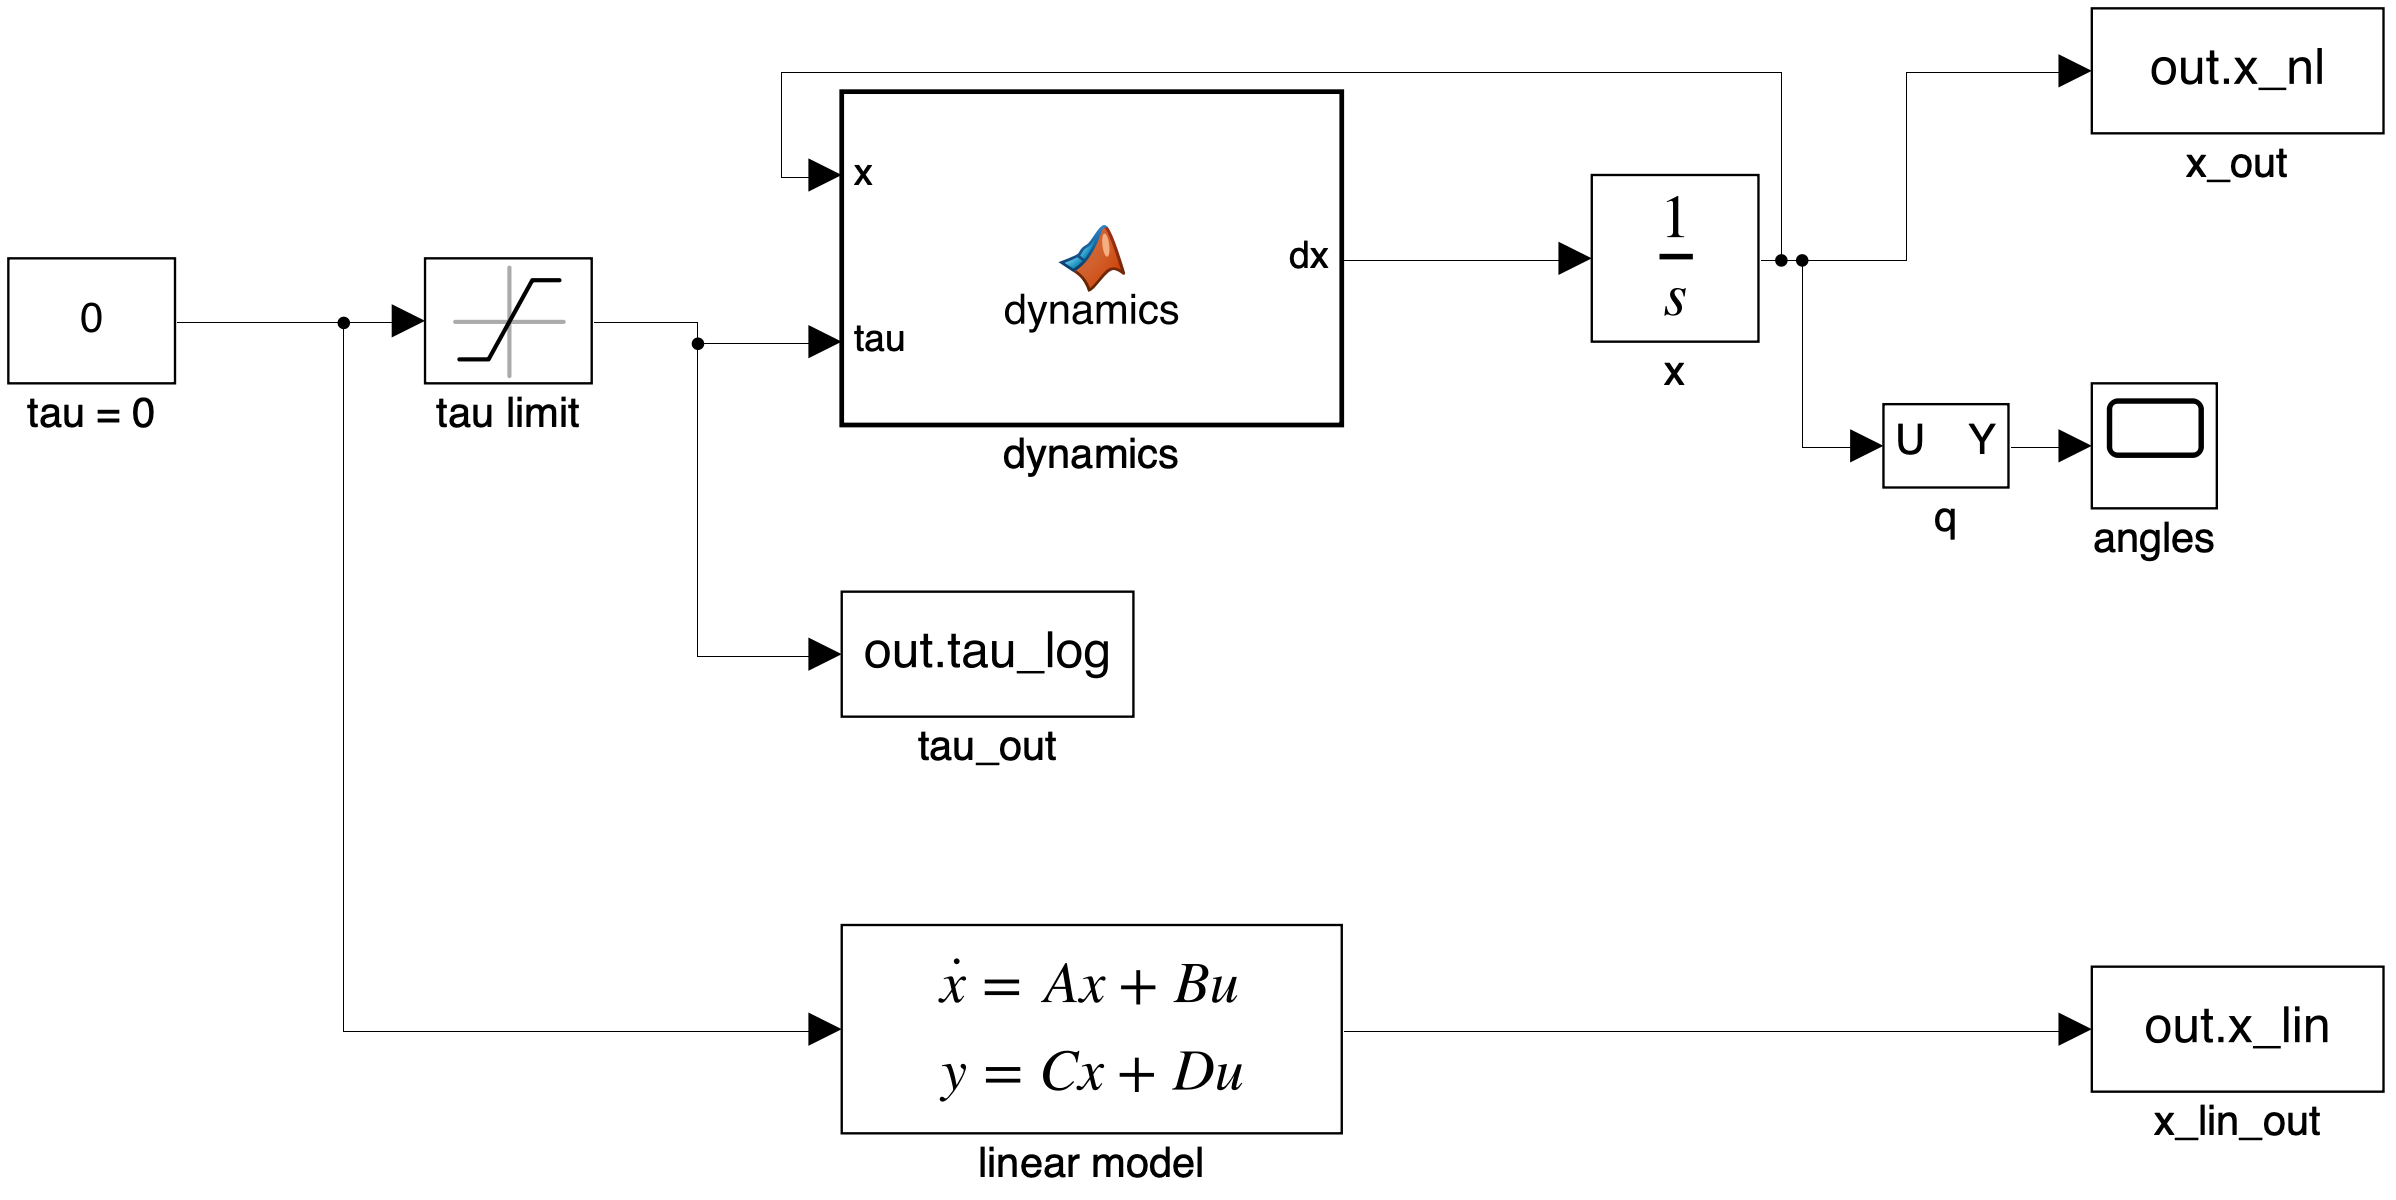
\includegraphics[width=0.82\textwidth]{figures/slx_openloop.png}
\caption{\texttt{Acrobot\_OpenLoop}: the nonlinear plant (top) and the linearized State-Space model (bottom) driven by the same $\tau=0$, so the two can be compared from the same deviation.}
\label{fig:slx_ol}
\end{figure}
\begin{figure}[H]
\centering
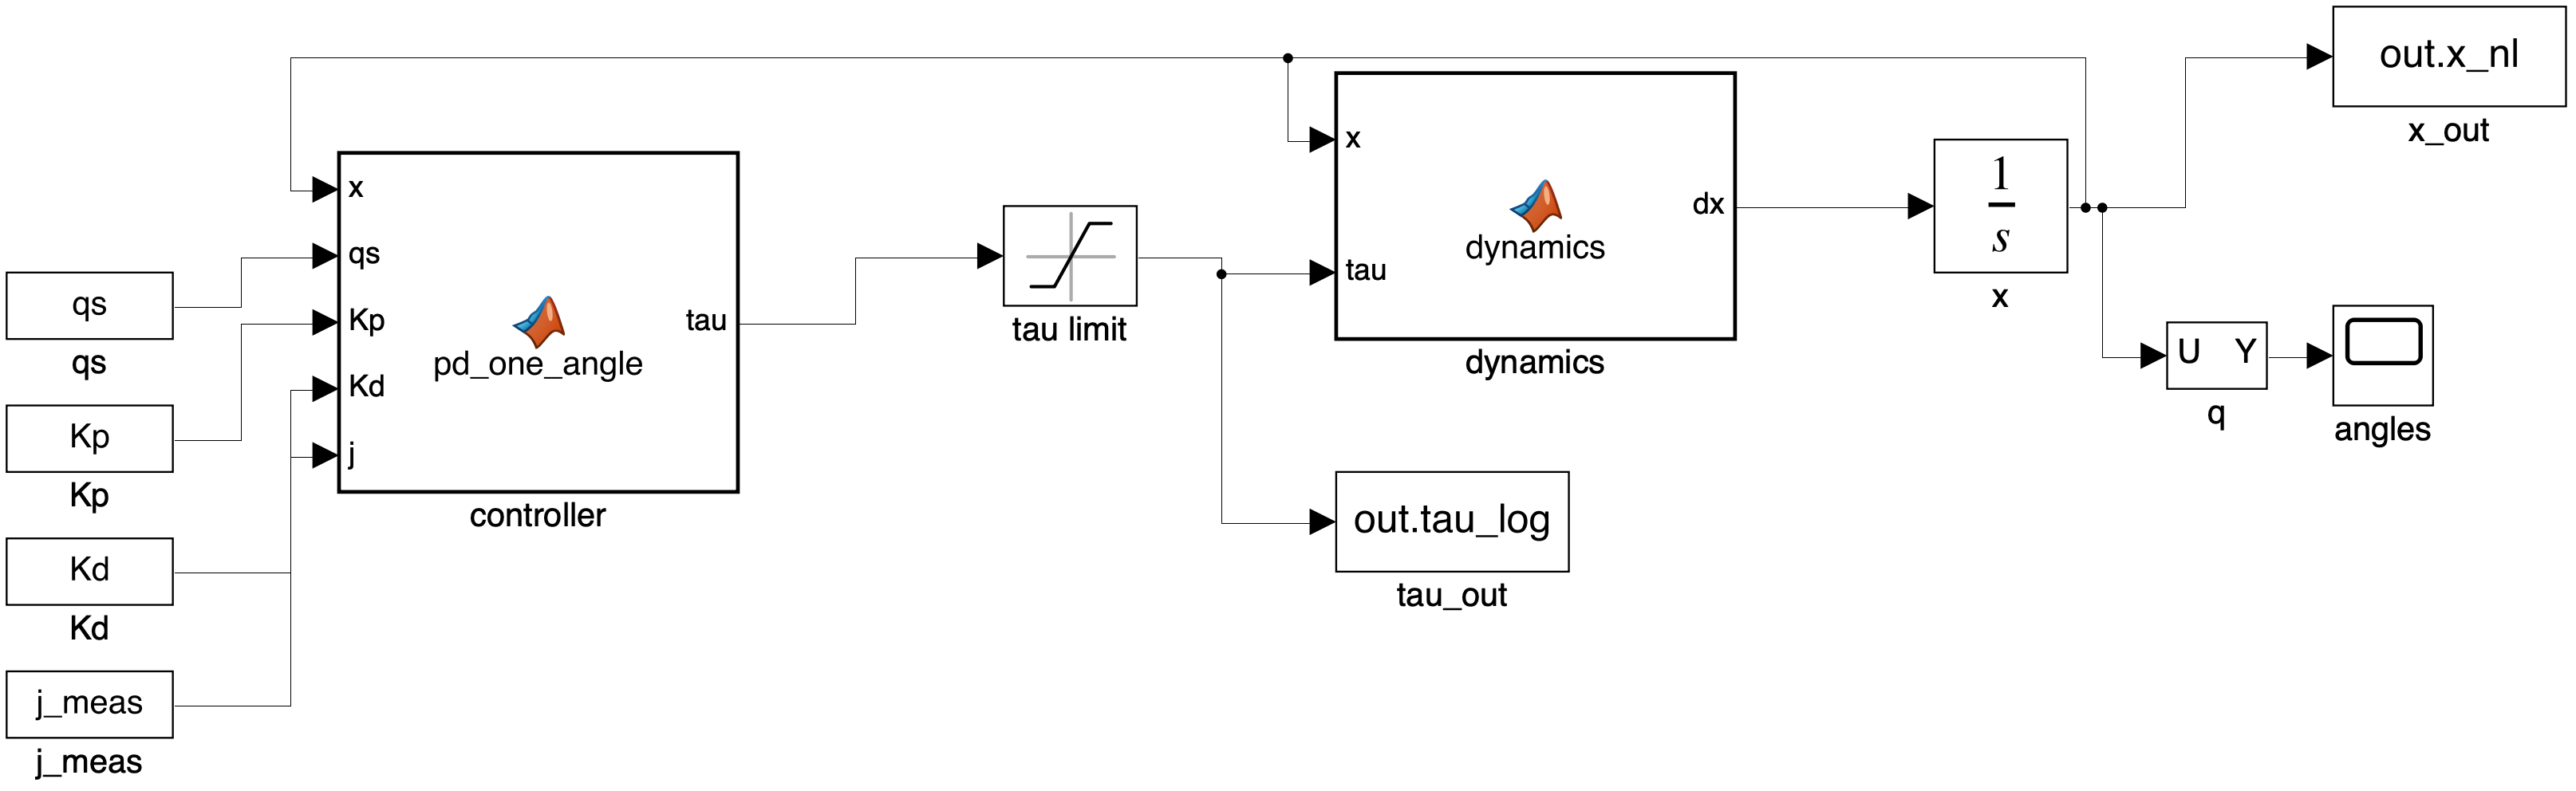
\includegraphics[width=\textwidth]{figures/slx_pd.png}
\caption{\texttt{Acrobot\_SingleAnglePD}: PD feedback from one measured angle (\texttt{j\_meas} $=1$ or $2$) at the upright.}
\label{fig:slx_pd}
\end{figure}
\begin{figure}[H]
\centering
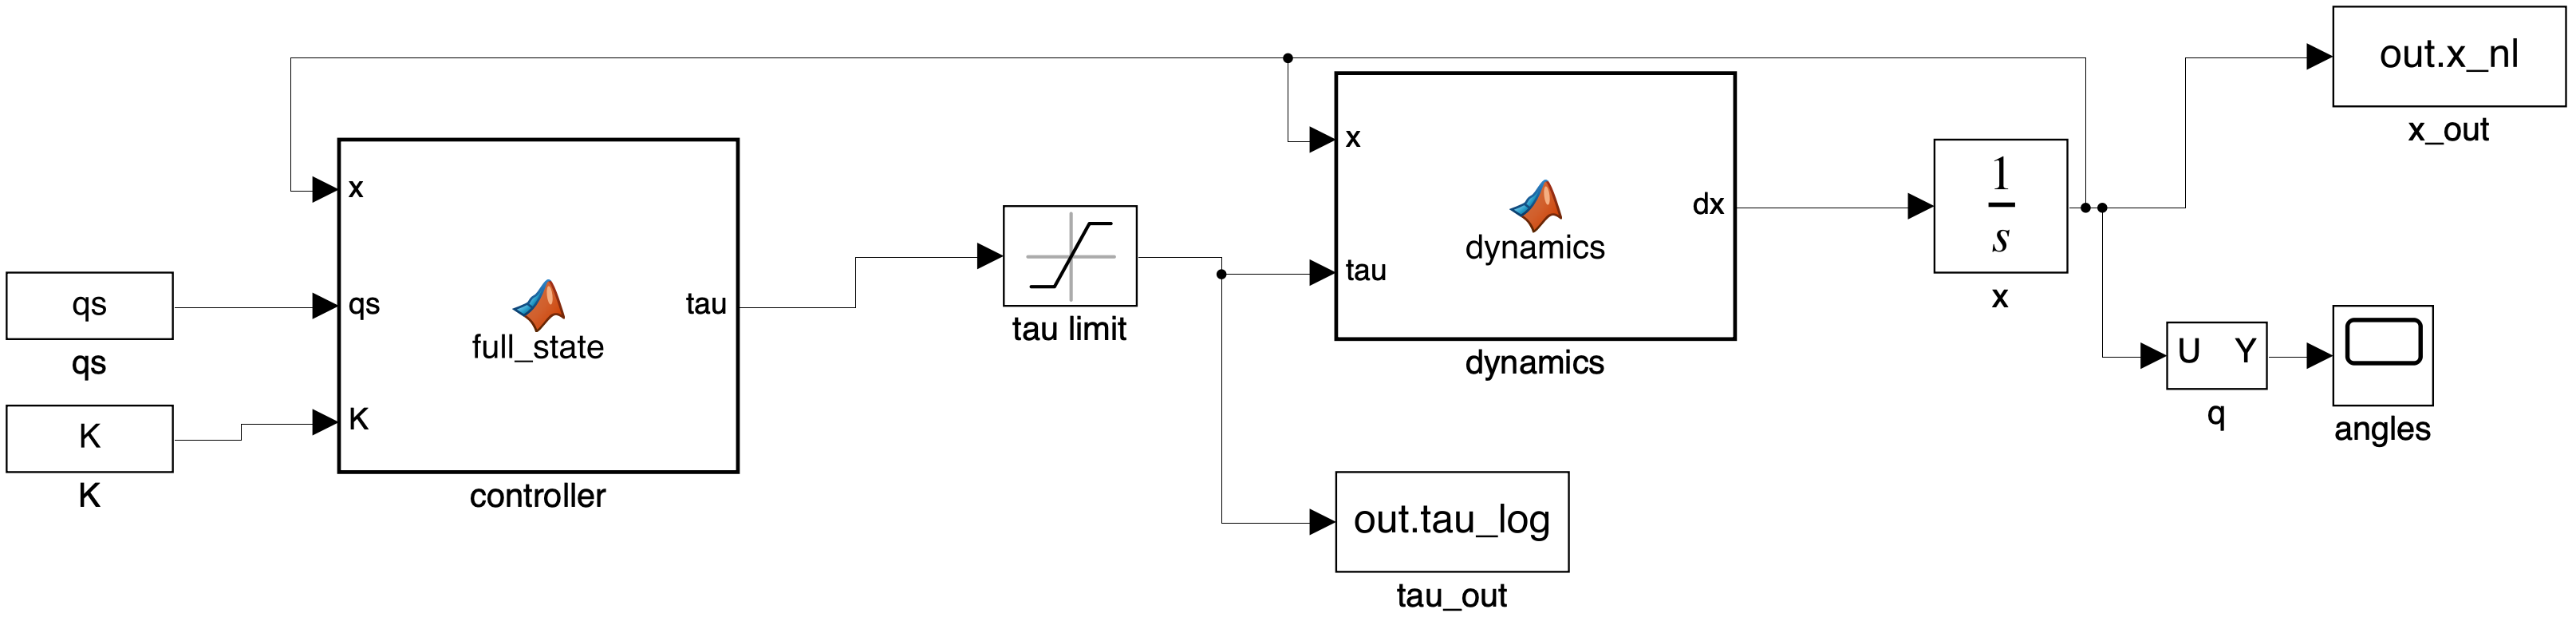
\includegraphics[width=\textwidth]{figures/slx_lqr.png}
\caption{\texttt{Acrobot\_LQR}: full-state feedback $\tau=\operatorname{sat}(-K\tilde x)$ about the equilibrium \texttt{qs}.}
\label{fig:slx_lqr}
\end{figure}
\begin{figure}[H]
\centering
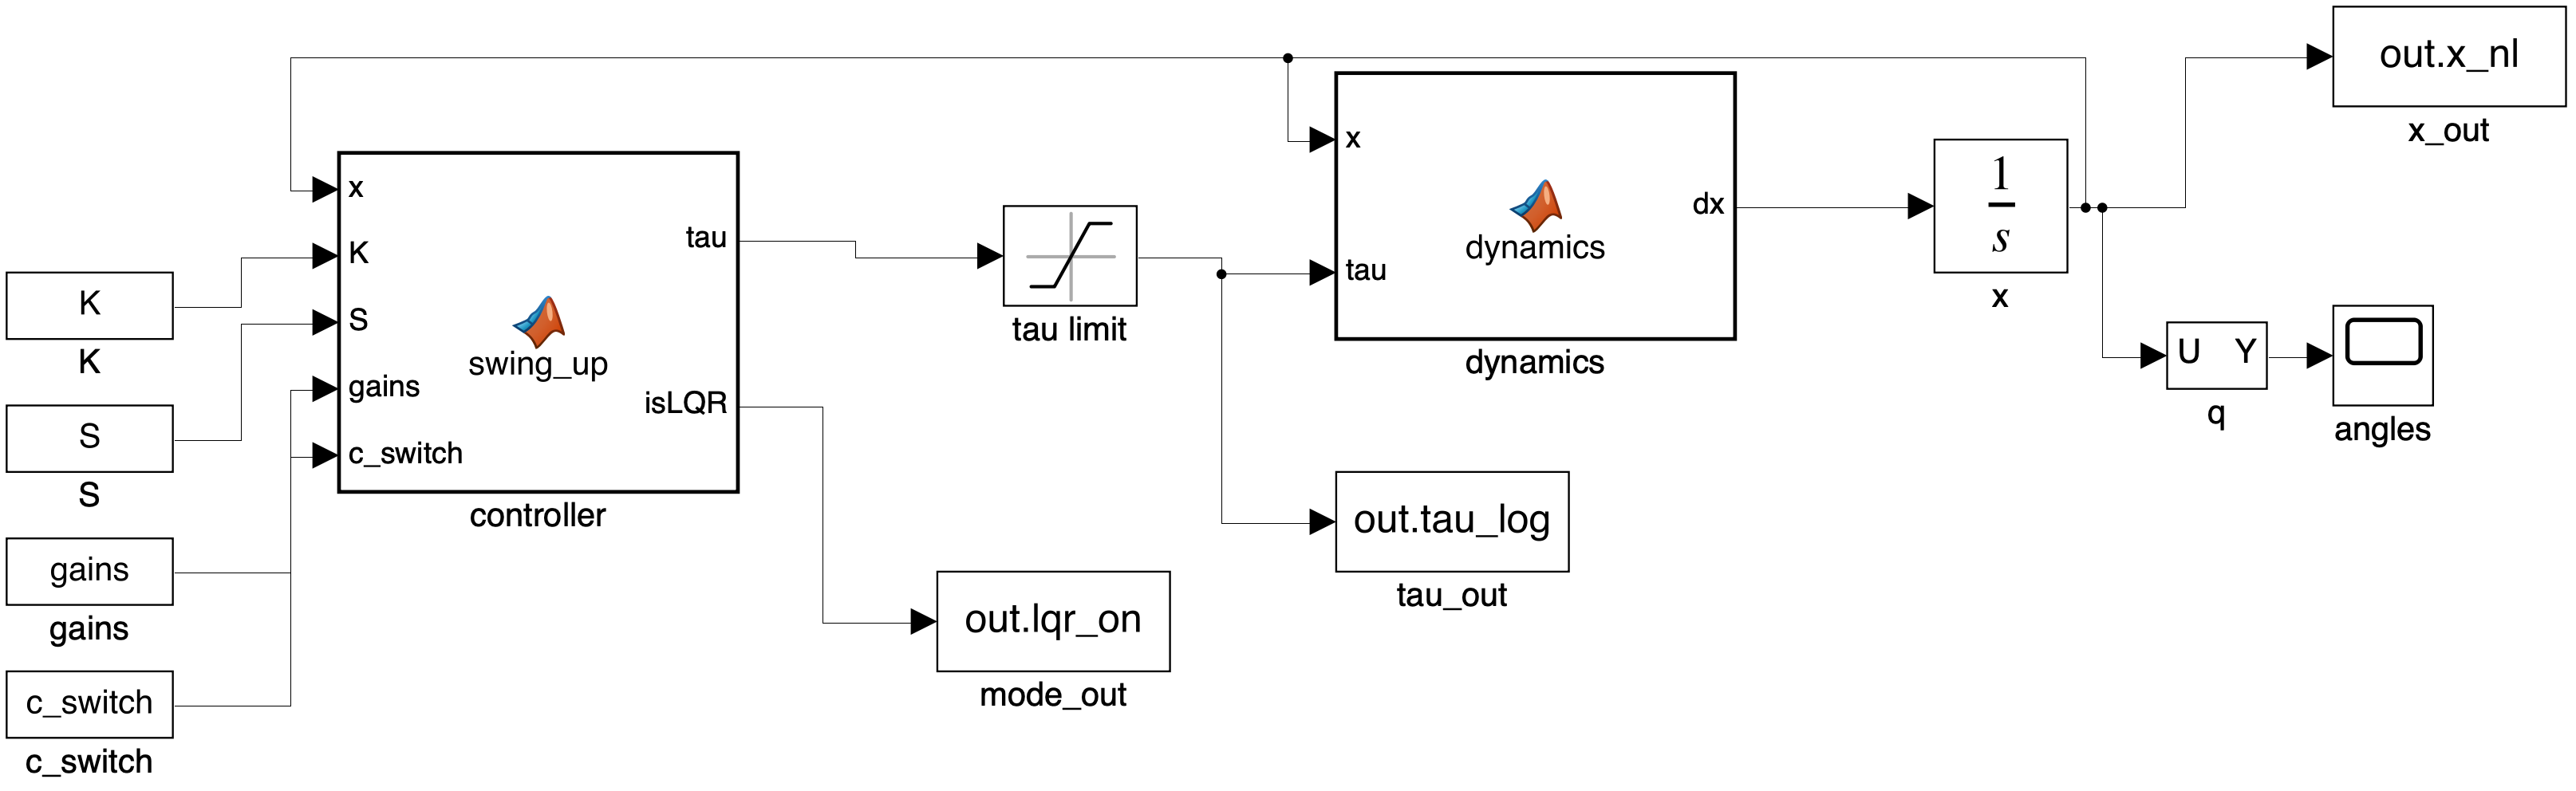
\includegraphics[width=\textwidth]{figures/slx_swingup.png}
\caption{\texttt{Acrobot\_SwingUp}: the hybrid controller has two outputs, the torque and the mode flag \texttt{isLQR} (logged as \texttt{lqr\_on}), which becomes 1 once the state enters the catch region $\tilde x^TS\tilde x<5$.}
\label{fig:slx_swing}
\end{figure}
In the swing-up model the controller block holds both laws of Section~\ref{sec:swing}. Outside the catch region it computes the energy error $E-E_{top}$ and the collocated partial-feedback-linearization torque; inside it applies the upright LQR. Because the switch is evaluated at every solver step, the solver handles the change of law as a discontinuity in $\tau$, exactly like the real hybrid controller.

\subsection{Results}
The script \texttt{run\_simulink\_models.m} simulates every model with the gains and initial states used in this report and checks each outcome. All 15 checks pass (Table~\ref{tab:slx}, Fig.~\ref{fig:slx_res}).
\begin{table}[H]
\centering
\caption{Simulink results (all checks pass)}
\label{tab:slx}
\resizebox{\textwidth}{!}{\begin{tabular}{|l|l|l|l|}
\hline
Model & Case & Simulink result & Expected (this report)\\ \hline
OpenLoop & $E_1$, from $(10^\circ,-10^\circ)$ & bounded, max.\ $14.7^\circ$ over 8 s & marginally stable\\
OpenLoop & $E_2$ & growth rate $3.171$ /s & pole $3.1775$ (error $0.19\%$)\\
OpenLoop & $E_3$ & growth rate $6.088$ /s & pole $6.1011$ (error $0.22\%$)\\
OpenLoop & $E_4$ & growth rate $4.300$ /s & pole $4.3010$ (error $0.03\%$)\\
SingleAnglePD & $E_3$, PD on $q_1$ ($K_p=-15$, $K_d=0$) & falls & no single-angle PD works\\
SingleAnglePD & $E_3$, PD on $q_2$ ($K_p=400$, $K_d=150$) & falls & no single-angle PD works\\
LQR & $E_3$, $R=0.03$, from $2^\circ$ & held, peak $|\tau|=17.56\Nm$ & held\\
LQR & $E_3$, from $5.5^\circ$ & held, $|\tau|$ saturates & held\\
LQR & $E_3$, from $7.5^\circ$ & falls & falls (beyond the $6^\circ$ limit)\\
LQR & $E_3$, from $(-10^\circ,25^\circ)$ & held, peak $3.34\Nm$ & held (centre-of-mass line)\\
LQR & $E_2$, $R=0.1$, from $(60^\circ,90^\circ)$ & held & held\\
LQR & $E_4$, $R=0.1$, from $(20^\circ,30^\circ)$ & held, peak $4.47\Nm$ & held\\
SwingUp & from $(3^\circ,0^\circ)$ & caught at $2.17$ s, held & caught at $2.17$ s\\
SwingUp & from $(0.5^\circ,0^\circ)$ & caught at $1.90$ s, held & held\\
SwingUp & from $(-10^\circ,20^\circ)$ & caught at $8.10$ s, held & held\\ \hline
\end{tabular}}
\end{table}
\begin{figure}[H]
\centering
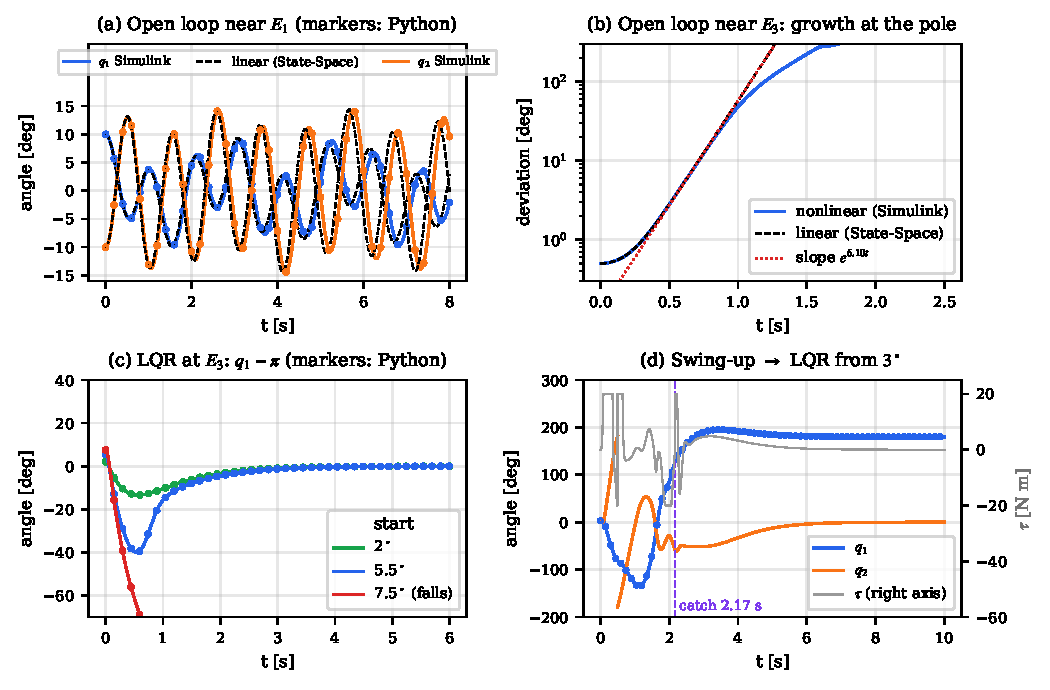
\includegraphics[width=\textwidth]{figures/fig_simulink.pdf}
\caption{Simulink responses (lines) with the Python simulation of the same case (markers). (a) Free oscillation near $E_1$, nonlinear vs.\ linear State-Space block. (b) Near $E_3$ the deviation grows at the unstable pole $6.10$/s until the nonlinearity takes over. (c) Upright LQR from $2^\circ$, $5.5^\circ$ and $7.5^\circ$. (d) Swing-up from $3^\circ$ and LQR catch at $2.17$ s, with the saturated torque (grey, right axis).}
\label{fig:slx_res}
\end{figure}

\subsection{Cross-Validation with the Python Model}
Each Simulink trajectory was re-simulated from the same initial state with the Python model and controllers used for the rest of the report, integrated independently with fixed-step RK4 (steps of at most 0.1~ms, landing exactly on the Simulink time points). The two implementations share only the equations, not the code or the solver.
\begin{table}[H]
\centering
\caption{Simulink vs.\ Python (maximum angle difference over the whole run)}
\label{tab:slxpy}
\resizebox{\textwidth}{!}{\begin{tabular}{|l|c|l|}
\hline
Case & Max.\ difference & Note\\ \hline
LQR gain $K$ (MATLAB vs.\ Python \texttt{lqr}) & $1.2\times10^{-13}$ (relative) & identical design\\
Open loop near $E_1$, 8 s & $6.9\times10^{-11}$ deg & smooth\\
Open loop near $E_3$, 2.5 s & $1.1\times10^{-10}$ deg & smooth; falls from $0.5^\circ$\\
LQR at $E_3$ from $2^\circ$ & $4.2\times10^{-11}$ deg & smooth\\
LQR at $E_3$ from $5.5^\circ$ & $6.0\times10^{-11}$ deg & saturates briefly\\
LQR at $E_3$ from $7.5^\circ$ & $0.17$ deg & both fall; long saturation\\
Swing-up from $3^\circ$, 10 s & $0.0066$ deg & catch $2.16691$ s vs.\ $2.16693$ s\\ \hline
\end{tabular}}
\end{table}
Where the torque is smooth the two agree to $10^{-10}$ degrees, which is the level of the integration error of the two solvers. They differ more (but still well below a degree) only where the torque is discontinuous: at saturation and at the swing-up/LQR switch. There the variable-step solver and the fixed-step RK4 place the corner at slightly different instants, and the difference is then amplified by the unstable dynamics. Even so, both give the same outcome in every case, and the swing-up catch times agree to $2\times10^{-5}$~s. The Simulink models therefore confirm the model, the stability results, the controllers and the swing-up independently of the Python and PyBullet code.

\subsection{Reproducing the Simulink Results}
The models are generated by a script rather than drawn by hand, so they can always be rebuilt identically:
\begin{itemize}
\item \texttt{build\_simulink\_models.m} creates the four \texttt{.slx} models and copies them into the code folders of the corresponding parts of the project;
\item \texttt{run\_simulink\_models.m} runs the 15 checks of Table~\ref{tab:slx} and prints PASS/FAIL;
\item \texttt{make\_simulink\_figures.m} exports the diagrams and the trajectories;
\item \texttt{compare\_with\_python.py} re-simulates them in Python and produces Table~\ref{tab:slxpy} and Fig.~\ref{fig:slx_res}.
\end{itemize}
Each model can also be opened and run by hand after setting its workspace inputs (Table~\ref{tab:slxmodels}).

% =====================================================================
\section{Software and Code}\label{sec:code}
% =====================================================================
\subsection{Files}
\begin{table}[H]
\centering
\caption{Code files}
\resizebox{\textwidth}{!}{\begin{tabular}{|l|l|l|}
\hline
Topic & File & Purpose\\ \hline
Model & \texttt{Acrobot\_Nonlinear\_Dynamics.m} & nonlinear model $\dot x=f(x,\tau)$ with the $20\Nm$ limit\\
Model & \texttt{Acrobot\_Linearize.m} & $A$, $B_\ell$ at an equilibrium\\
Stability & \texttt{Acrobot\_Phase2\_Main.m} & poles, zeros, ranks, verdicts, growth rates, single-angle PD test\\
Control & \texttt{Acrobot\_Phase3\_Design.m}, \texttt{Acrobot\_Phase3\_Main.m} & controllers, guaranteed regions, regions of attraction\\
Swing-up & \texttt{Acrobot\_Phase4\_Controller.m}, \texttt{Acrobot\_Phase4\_Main.m} & hybrid controller, swing-up and robustness tests\\
Learned swing-up & \texttt{acrobot\_env.py}, \texttt{train.py}, \texttt{evaluate.py} & environment, SAC training, comparison (Python)\\
Simulator & \texttt{acrobot\_phase\{2,3,4\}\_sim.py} & interactive PyBullet dashboards\\
Simulink & \texttt{Acrobot\_OpenLoop.slx}, \texttt{Acrobot\_SingleAnglePD.slx} & open loop vs.\ linear model; single-angle PD\\
Simulink & \texttt{Acrobot\_LQR.slx}, \texttt{Acrobot\_SwingUp.slx} & full-state LQR; hybrid swing-up $\to$ LQR\\
Simulink & \texttt{build\_simulink\_models.m}, \texttt{run\_simulink\_models.m} & build the models; run the 15 checks\\
Simulink & \texttt{make\_simulink\_figures.m}, \texttt{compare\_with\_python.py} & diagrams, trajectories, Simulink vs.\ Python\\ \hline
\end{tabular}}
\end{table}
\subsection{Pseudo-Code}
\begin{algorithm}[H]
\caption{Nonlinear dynamics $\dot x=f(x,\tau)$ (\texttt{Acrobot\_Nonlinear\_Dynamics.m}) and linearization (\texttt{Acrobot\_Linearize.m})}
\label{alg:model}
\begin{algorithmic}[1]
\Function{Dynamics}{$x=[q_1,q_2,\dot q_1,\dot q_2]$, $\tau$}
  \State $\tau\gets\max(-20,\min(20,\tau))$ \Comment{motor limit}
  \State build $M(q)$, $C(q,\dot q)$ and $\tau_g(q)$ from the given model
  \State solve $M\,\ddot q=\tau_g+B\tau-C\dot q$ for $\ddot q$ \Comment{backslash, never $M^{-1}$}
  \State \Return $[\dot q;\ \ddot q]$
\EndFunction
\Function{Linearize}{$q^*$}
  \State $K\gets\partial\tau_g/\partial q$ at $q^*$; \quad $P\gets M(q^*)^{-1}K$; \quad $r\gets M(q^*)^{-1}B$
  \State \Return $A=\begin{bmatrix}0&I\\P&0\end{bmatrix}$, $B_\ell=\begin{bmatrix}0\\r\end{bmatrix}$
\EndFunction
\end{algorithmic}
\end{algorithm}

\begin{algorithm}[H]
\caption{Stability analysis and single-angle test (\texttt{Acrobot\_Phase2\_Main.m})}
\label{alg:p2}
\begin{algorithmic}[1]
\For{each equilibrium $E_k\in\{E_1,E_2,E_3,E_4\}$}
  \State $(A,B_\ell)\gets$ \Call{Linearize}{$q^*_k$}; \quad poles $\gets\operatorname{eig}(A)$
  \State $G_1,G_2\gets$ transfer functions $\tau\to q_1$, $\tau\to q_2$; \quad zeros $\gets$ roots of their numerators
  \State check $\operatorname{rank}\mathcal C=\operatorname{rank}\mathcal O_1=\operatorname{rank}\mathcal O_2=4$ \Comment{minimal: poles of $G_j$ = eig$(A)$}
  \State verdict $\gets$ asymptotically / marginally stable / unstable from the signs of $\operatorname{Re}(\text{poles})$
\EndFor
\For{$E_k\in\{E_2,E_3,E_4\}$} \Comment{nonlinear check}
  \State simulate $\tau=0$ from a $0.01^\circ$ offset (\texttt{ode45})
  \State fit the slope of $\ln\|\tilde q(t)\|$ and compare it with the largest RHP pole
\EndFor
\For{measured angle $j\in\{1,2\}$ at $E_3$} \Comment{PD from one angle}
  \State write $G_j=(b_2s^2+b_0)/\Delta(s)$
  \If{$b_2\,b_0<0$} \State PD is impossible (no Hurwitz $K_p,K_d$) \EndIf
  \State grid-search $(K_p,K_d)$: record the smallest $\max\operatorname{Re}\lambda(A-B_\ell F)$
\EndFor
\end{algorithmic}
\end{algorithm}

\begin{algorithm}[H]
\caption{Controller design and limits (\texttt{Acrobot\_Phase3\_Design.m}, \texttt{Acrobot\_Phase3\_Main.m})}
\label{alg:p3}
\begin{algorithmic}[1]
\For{each design (LQR at $E_2,E_3,E_4$; pole placement at $E_3$; elbow PD at $E_1$)}
  \State $(A,B_\ell)\gets$ \Call{Linearize}{$q^*$}
  \If{LQR} \State $(K,S)\gets\texttt{lqr}(A,B_\ell,Q=I,R)$; \quad $c^*\gets\tau_{\max}^2/(KS^{-1}K^T)$ \Comment{guaranteed region}
  \ElsIf{pole placement} \State $K\gets\texttt{place}(A,B_\ell,\{-3,-4,-5,-6\})$
  \Else \State $K\gets[0,\ K_p,\ 0,\ K_d]$ \Comment{elbow angle only}
  \EndIf
  \State print $K$ and $\operatorname{eig}(A-B_\ell K)$
\EndFor
\Function{RegionOfAttraction}{$K$, $q^*$, grid of $(\tilde q_1(0),\tilde q_2(0))$}
  \For{each grid point}
    \State simulate $\tau=\operatorname{sat}(-K\tilde x)$ for 10 s from rest \Comment{nonlinear model}
    \State mark it recovered if it ends within $1^\circ$ and $0.05$ rad/s of $q^*$
  \EndFor
  \State \Return the map, the share recovered and the largest offset along each axis
\EndFunction
\end{algorithmic}
\end{algorithm}

\begin{algorithm}[H]
\caption{Hybrid swing-up controller (\texttt{Acrobot\_Phase4\_Controller.m}) and tests (\texttt{Acrobot\_Phase4\_Main.m})}
\label{alg:p4}
\begin{algorithmic}[1]
\Function{Controller}{$x$}
  \State $\tilde x\gets$ deviation of $x$ from the upright $E_3$ (angles wrapped to $\pm\pi$)
  \If{$\tilde x^TS\tilde x<c_{sw}=5$}
    \State $\tau\gets-K\tilde x$ \Comment{catch: upright LQR}
  \Else \Comment{swing-up: energy pumping}
    \State $E\gets\frac12\dot q^TM\dot q+U(q)$
    \State $v\gets-k_1\tilde q_2-k_2\dot q_2+k_3\,\dot q_1\,(E-E_{top})$
    \State $\tau\gets(M_{22}-M_{21}M_{12}/M_{11})\,v+h_2-M_{21}h_1/M_{11}$ \Comment{partial feedback linearization}
  \EndIf
  \State \Return $\operatorname{sat}(\tau)$ \Comment{$|\tau|\le20\Nm$}
\EndFunction
\For{each start (three chosen starts, then 40 random starts near hanging)}
  \State simulate with fixed-step RK4 (1 ms) for 30--40 s, calling \Call{Controller}{} every step
  \State record the first catch time, the share of time at $|\tau|=20$, and whether $E_3$ is held
\EndFor
\end{algorithmic}
\end{algorithm}

\begin{algorithm}[H]
\caption{Learned swing-up: environment step and SAC training (\texttt{acrobot\_env.py}, \texttt{train.py})}
\label{alg:p5train}
\begin{algorithmic}[1]
\Function{Reset}{}
  \State $x\gets$ random start near hanging; \quad $m_1,m_2\gets1$ kg \Comment{robust policy: $m_i\sim U[0.7,1.3]$ kg}
\EndFunction
\Function{EnvStep}{$x$, action $a\in[-1,1]$}
  \State $\tau\gets20a$; \quad integrate the model with masses $m_1,m_2$ for 20 ms (four RK4 steps of 5 ms)
  \State $r\gets-((E-E_{top})/E_{top})^2-0.3(1+\cos q_1)-0.1(1-\cos q_2)-0.001(\tau/20)^2$
  \If{$\tilde x^TS\tilde x<5$} \State $r\gets r+100$; episode ends \Comment{reached the LQR catch zone}
  \EndIf
  \State $o\gets[\cos q_1,\sin q_1,\cos q_2,\sin q_2,\dot q_1/10,\dot q_2/10]$ \Comment{robust policy: append $(E_{top}-E)/E_{top}$}
  \State \Return $o$, $r$
\EndFunction
\State initialise actor $\pi_\theta$, critics $Q_{\phi_1},Q_{\phi_2}$ (2$\times$256 each), empty replay buffer
\For{$10^6$ environment steps (4 environments in parallel)}
  \State $a\sim\pi_\theta(\cdot\mid o)$; \quad $(o',r)\gets$ \Call{EnvStep}{$x,a$}; \quad store $(o,a,r,o')$ in the buffer
  \State sample a batch of 256; update the critics towards $r+\gamma(\min_iQ_{\phi_i}(o',a')-\alpha\log\pi_\theta(a'\mid o'))$
  \State update the actor to maximise $\min_iQ_{\phi_i}(o,a)-\alpha\log\pi_\theta(a\mid o)$; tune $\alpha$
\EndFor
\State save $\pi_\theta$
\end{algorithmic}
\end{algorithm}
\begin{algorithm}[H]
\caption{Learned swing-up: RL $\to$ LQR controller and evaluation (\texttt{acrobot\_env.py}, \texttt{evaluate.py})}
\label{alg:p5eval}
\begin{algorithmic}[1]
\Function{RLController}{$x$}
  \If{$\tilde x^TS\tilde x<5$} \State \Return $\operatorname{sat}(-K\tilde x)$ \Comment{same upright LQR catch}
  \EndIf
  \State every 20 ms: $\tau\gets20\,\pi_\theta(o)$ (deterministic); hold it in between
  \State \Return $\tau$
\EndFunction
\For{link masses $\in\{0.6,\ 0.8,\ 1.0,\ 1.2,\ 1.4\}$ kg} \Comment{controllers always assume 1 kg}
  \For{each of the 40 random starts, for the energy and both RL controllers}
    \State simulate 30 s; record held, first catch time, torque saturation, elbow work and hand-overs
  \EndFor
\EndFor
\end{algorithmic}
\end{algorithm}

\subsection{Animations}
2K Manim animations of the work:
\href{https://drive.google.com/file/d/18Ic6QdsY37QBfvFIwmVA_8Z-u4AyNPdg/view?usp=sharing}{\textcolor{blue}{model and equilibria}},
\href{https://drive.google.com/file/d/19THfoXXzbdMtbteCKE4v0VRLpV869wE0/view?usp=sharing}{\textcolor{blue}{stability}},
\href{https://drive.google.com/file/d/1c-7Yy664ZP4TCJIeDbrAmFozHC8frao1/view?usp=sharing}{\textcolor{blue}{control}},
\href{https://drive.google.com/file/d/1jPQRn3W-bvUyvSKlHvYmX74bfPX9N16P/view?usp=sharing}{\textcolor{blue}{swing-up}};
the comparison of the learned and energy swing-ups is \url{phase5_rl/RL_vs_Energy_SwingUp_2K.mp4}.

% =====================================================================
\section{Tabulation}
% =====================================================================
\begin{table}[H]
\centering
\caption{Summary of the stability analysis}
\begin{tabular}{|c|c|c|c|}
\hline
Equilibrium & RHP poles & Energy shape & Stability\\ \hline
$E_1$ down--down & 0 & minimum & marginally (Lyapunov) stable\\
$E_2$ down--up & 1 & saddle & unstable\\
$E_3$ up--up & 2 & maximum & unstable\\
$E_4$ up--down & 1 & saddle & unstable\\ \hline
\end{tabular}
\end{table}
\begin{table}[H]
\centering
\caption{Summary of every controller ($|\tau|\le20\Nm$)}
\resizebox{\textwidth}{!}{\begin{tabular}{|l|l|l|}
\hline
Controller & Works? & Limit\\ \hline
PD on one angle at $E_3$ & no (proved) & always unstable\\
Observer + LQR, one angle, at $E_3$ & yes & $1.42^\circ$ ($q_1$), $0.23^\circ$ ($q_2$)\\
Full-state LQR at $E_3$ & yes & $6^\circ$ / $13^\circ$, $\ge43^\circ$ along the CoM line\\
Pole placement at $E_3$ & yes & $5^\circ$ / $9^\circ$\\
LQR at $E_2$ & yes & almost any rest position (99.7\%)\\
LQR at $E_4$ & yes & $35^\circ$ / $55^\circ$\\
Elbow PD at $E_1$ & yes & 78\% of $\pm180^\circ$\\
Energy swing-up $\to$ LQR & yes & 39/40 random starts (40 s), 35/40 (30 s)\\
RL (SAC) swing-up $\to$ LQR, 1 kg only & yes & 40/40 (30 s); 15/40 with links $+20\%$ heavier\\
RL swing-up $\to$ LQR, random masses & yes & 40/40 from 0.6 to 1.2 kg; 2/40 at 1.4 kg\\ \hline
\end{tabular}}
\end{table}

% =====================================================================
\section{Conclusion}
% =====================================================================
The given acrobot model was verified from first principles. It has four zero-torque equilibria, all with both links vertical. Only the hanging pose is stable, and only in the Lyapunov sense: with no friction it oscillates forever. The other three are unstable, with one, two and one right-half-plane poles, matching the number of directions in which the potential energy decreases. The transfer functions and the state matrix agree because every realization is minimal, and PyBullet confirmed the predicted growth rates to within $0.25\%$.

A single measured angle cannot stabilize the upright with PD feedback, because the transfer functions have real right-half-plane zeros. An observer-based controller can, but only for about a degree. With full-state feedback all four equilibria were stabilized. At the upright the $20\Nm$ limit, not the tuning, restricts LQR to a thin band around the line where the centre of mass is over the pivot.

An energy-pumping swing-up with partial feedback linearization brings the arm from hanging to the upright, and the LQR catches and holds it from 39 of 40 random starts. Stiffer gains fail because saturation breaks the linearization. A swing-up learned with reinforcement learning was faster, gentler and more reliable on the model it was trained on, but much less robust when the link masses changed. Training it on random link masses, with the missing energy as one extra input, fixed this over the practised range (40 of 40 from 0.6 to 1.2~kg) at no cost on the correct model; far outside that range (1.4~kg) the physics-based law remained the more reliable one. The hybrid design (learn or design the swing-up, keep the provable LQR catch) proved the most useful structure throughout.

Finally, every model and controller except the learned one was rebuilt in Simulink. The Simulink models pass all 15 checks and agree with the independent Python simulation to $10^{-10}$ degrees wherever the torque is smooth, and to well below a degree across saturation and the swing-up switch, so the results do not depend on one particular piece of code.

% =====================================================================
\section{Contributions}
% =====================================================================
% Fill in who did what before submitting.
\begin{enumerate}
\item Report compilation -- \underline{\hspace{4cm}}
\item Modelling, equilibria and linearization (Sections 2--4) -- \underline{\hspace{4cm}}
\item Simulation environment and verification (Section 5) -- \underline{\hspace{4cm}}
\item Stability analysis and single-sensor feedback (Sections 6--7) -- \underline{\hspace{4cm}}
\item Controller design and limits (Sections 8--9) -- \underline{\hspace{4cm}}
\item Swing-up control (Section 10) -- \underline{\hspace{4cm}}
\item Learning-based swing-up (Section 11) -- \underline{\hspace{4cm}}
\item Simulink models and cross-validation (Section 12) -- \underline{\hspace{4cm}}
\item Code, simulator and animations (Section 13) -- \underline{\hspace{4cm}}
\end{enumerate}

\begin{thebibliography}{9}
\bibitem{spong} M.~W. Spong, ``The swing up control problem for the Acrobot,'' \emph{IEEE Control Systems Magazine}, vol.~15, no.~1, pp.~49--55, 1995.
\bibitem{tedrake} R.~Tedrake, \emph{Underactuated Robotics}, MIT, 2024. Available: https://underactuated.csail.mit.edu
\bibitem{skogestad} S.~Skogestad and I.~Postlethwaite, \emph{Multivariable Feedback Control}, 2nd ed., Wiley, 2005.
\bibitem{khalil} H.~K. Khalil, \emph{Nonlinear Systems}, 3rd ed., Prentice Hall, 2002.
\bibitem{pybullet} E.~Coumans and Y.~Bai, ``PyBullet, a Python module for physics simulation,'' 2016--2024. Available: https://pybullet.org
\bibitem{youla} D.~C. Youla, J.~J. Bongiorno and C.~N. Lu, ``Single-loop feedback-stabilization of linear multivariable dynamical plants,'' \emph{Automatica}, vol.~10, pp.~159--173, 1974.
\bibitem{anderson} B.~D.~O. Anderson and J.~B. Moore, \emph{Optimal Control: Linear Quadratic Methods}, Prentice Hall, 1990.
\bibitem{sac} T.~Haarnoja, A.~Zhou, P.~Abbeel and S.~Levine, ``Soft actor-critic: Off-policy maximum entropy deep reinforcement learning with a stochastic actor,'' in \emph{Proc. ICML}, 2018.
\bibitem{sb3} A.~Raffin, A.~Hill, A.~Gleave, A.~Kanervisto, M.~Ernestus and N.~Dormann, ``Stable-Baselines3: Reliable reinforcement learning implementations,'' \emph{JMLR}, vol.~22, no.~268, pp.~1--8, 2021.
\end{thebibliography}

\end{document}
